%!TEX TS-program = xelatex
%!TEX encoding = UTF-8 Unicode
\documentclass[a4paper,10pt,twosided]{book}
\usepackage[polish]{babel}
\usepackage{fontspec}
\usepackage{hyperref}
\usepackage{fancyhdr}
\usepackage{fancyref}
\usepackage{wrapfig}
\usepackage{geometry}
\usepackage{tabularx}
\usepackage{ifthen}
\usepackage{textcomp}
\usepackage{array}
\usepackage[compact]{titlesec}
\usepackage[section]{placeins}
\defaultfontfeatures{Ligatures=TeX}
\setmainfont{Liberation Serif}
\hypersetup{
    colorlinks=true,
    linkcolor=blue,
    urlcolor=blue
}

\graphicspath{ {images/} }

\newcommand{\declarepagestyle}[0]{
\fancyhead[LE,RO]{\thepage}
\fancyfoot{}
\renewcommand{\headrulewidth}{0.4pt}
\renewcommand{\footrulewidth}{0.4pt}
}

\fancypagestyle{plain}{\declarepagestyle}

\fancypagestyle{empty}{%
\fancyhead{}
\fancyfoot{}
\renewcommand{\headrulewidth}{0pt}
\renewcommand{\footrulewidth}{0pt}
}

\newcommand{\refwithpage}[3]{
\ref{#1}\ifthenelse{\equal{\thepage}{\pageref{#1}}}{}{#2\pageref{#1}#3}%
}

\newcommand{\pref}[1]{\refwithpage{#1}{ (strona }{)}}
\newcommand{\ppref}[1]{\refwithpage{#1}{ -- strona }{}}
%\newcommand{\pref}[1]{\ref{#1} (strona \pageref{#1})}
%\newcommand{\ppref}[1]{\ref{#1} -- strona \pageref{#1}}

\pagestyle{fancy}
\declarepagestyle
\setlength{\headheight}{15pt}
\begin{document}

\newgeometry{margin=2cm}
\thispagestyle{empty}
\begin{titlepage}
{\centering
\noindent
\includegraphics[width=\textwidth]{eu_logo.png}

\hrulefill

\vspace{\fill}
\noindent
\includegraphics[width=0.75\textwidth]{app_logo.pdf}

\vspace{-3cm}
\noindent\LARGE Platforma Testów IBE\par%
\noindent\large instrukcja obsługi aplikacji\par%
\vspace{10cm}
\noindent\Large Mariusz Pluciński, Speednet Sp. z o.o.\par%
\vspace{2cm}
\noindent\Large 15 maja 2014\par%
\vspace{\fill}
}
\end{titlepage}
\restoregeometry

\tableofcontents


\chapter{Uruchamianie aplikacji}
\label{chap:launch}

\begin{wrapfigure}{r}{0.5\textwidth}
\vspace{-1em}

\includegraphics[width=0.48\textwidth]{activity_launch-first.png}
\caption{Komunikat o uruchamianiu aplikacji po raz pierwszy}
\label{fig:launch_firstrun}
\end{wrapfigure}

Po wybraniu ikony aplikacji z pulpitu, bądź systemowej listy zainstalowanych aplikacji, następuje proces uruchamiania aplikacji.

Gdy aplikacja uruchamiana jest po raz pierwszy, jej uruchomienie może zająć więcej czasu. Wyświetlany jest wówczas obraz jak na rysunku \pref{fig:launch_firstrun}. Jest to spowodowane instalacją na urządzeniu demonstracyjnych banków zadań. Operacja ta może trwać nawet powyżej jednej minuty, i nie powinna być przerywana.

Kolejne uruchomienia aplikacji nie wymagają przeprowadzenia takiego procesu i nie trwają więcej niż kilka sekund. Wyświetlany jest wówczas obraz jak na rysunku \pref{fig:launch_normalrun}

\begin{wrapfigure}{l}{0.5\textwidth}

\includegraphics[width=0.48\textwidth]{activity_launch-normal.png}
\caption{Komunikat o uruchamianiu aplikacji}
\label{fig:launch_normalrun}
\end{wrapfigure}


\chapter{Ekran logowania}
\label{chap:login}

Ekran logowania aplikacji jest punktem startowym dla użytkownika. Daje dostęp do funkcji nie wymagających logowania, oraz umożliwia przejście do dalszych ekranów aplikacji. Ekran ten wygląda jak na rysunku \pref{fig:login}.

\begin{figure}[h]
\vspace{-0.5em}
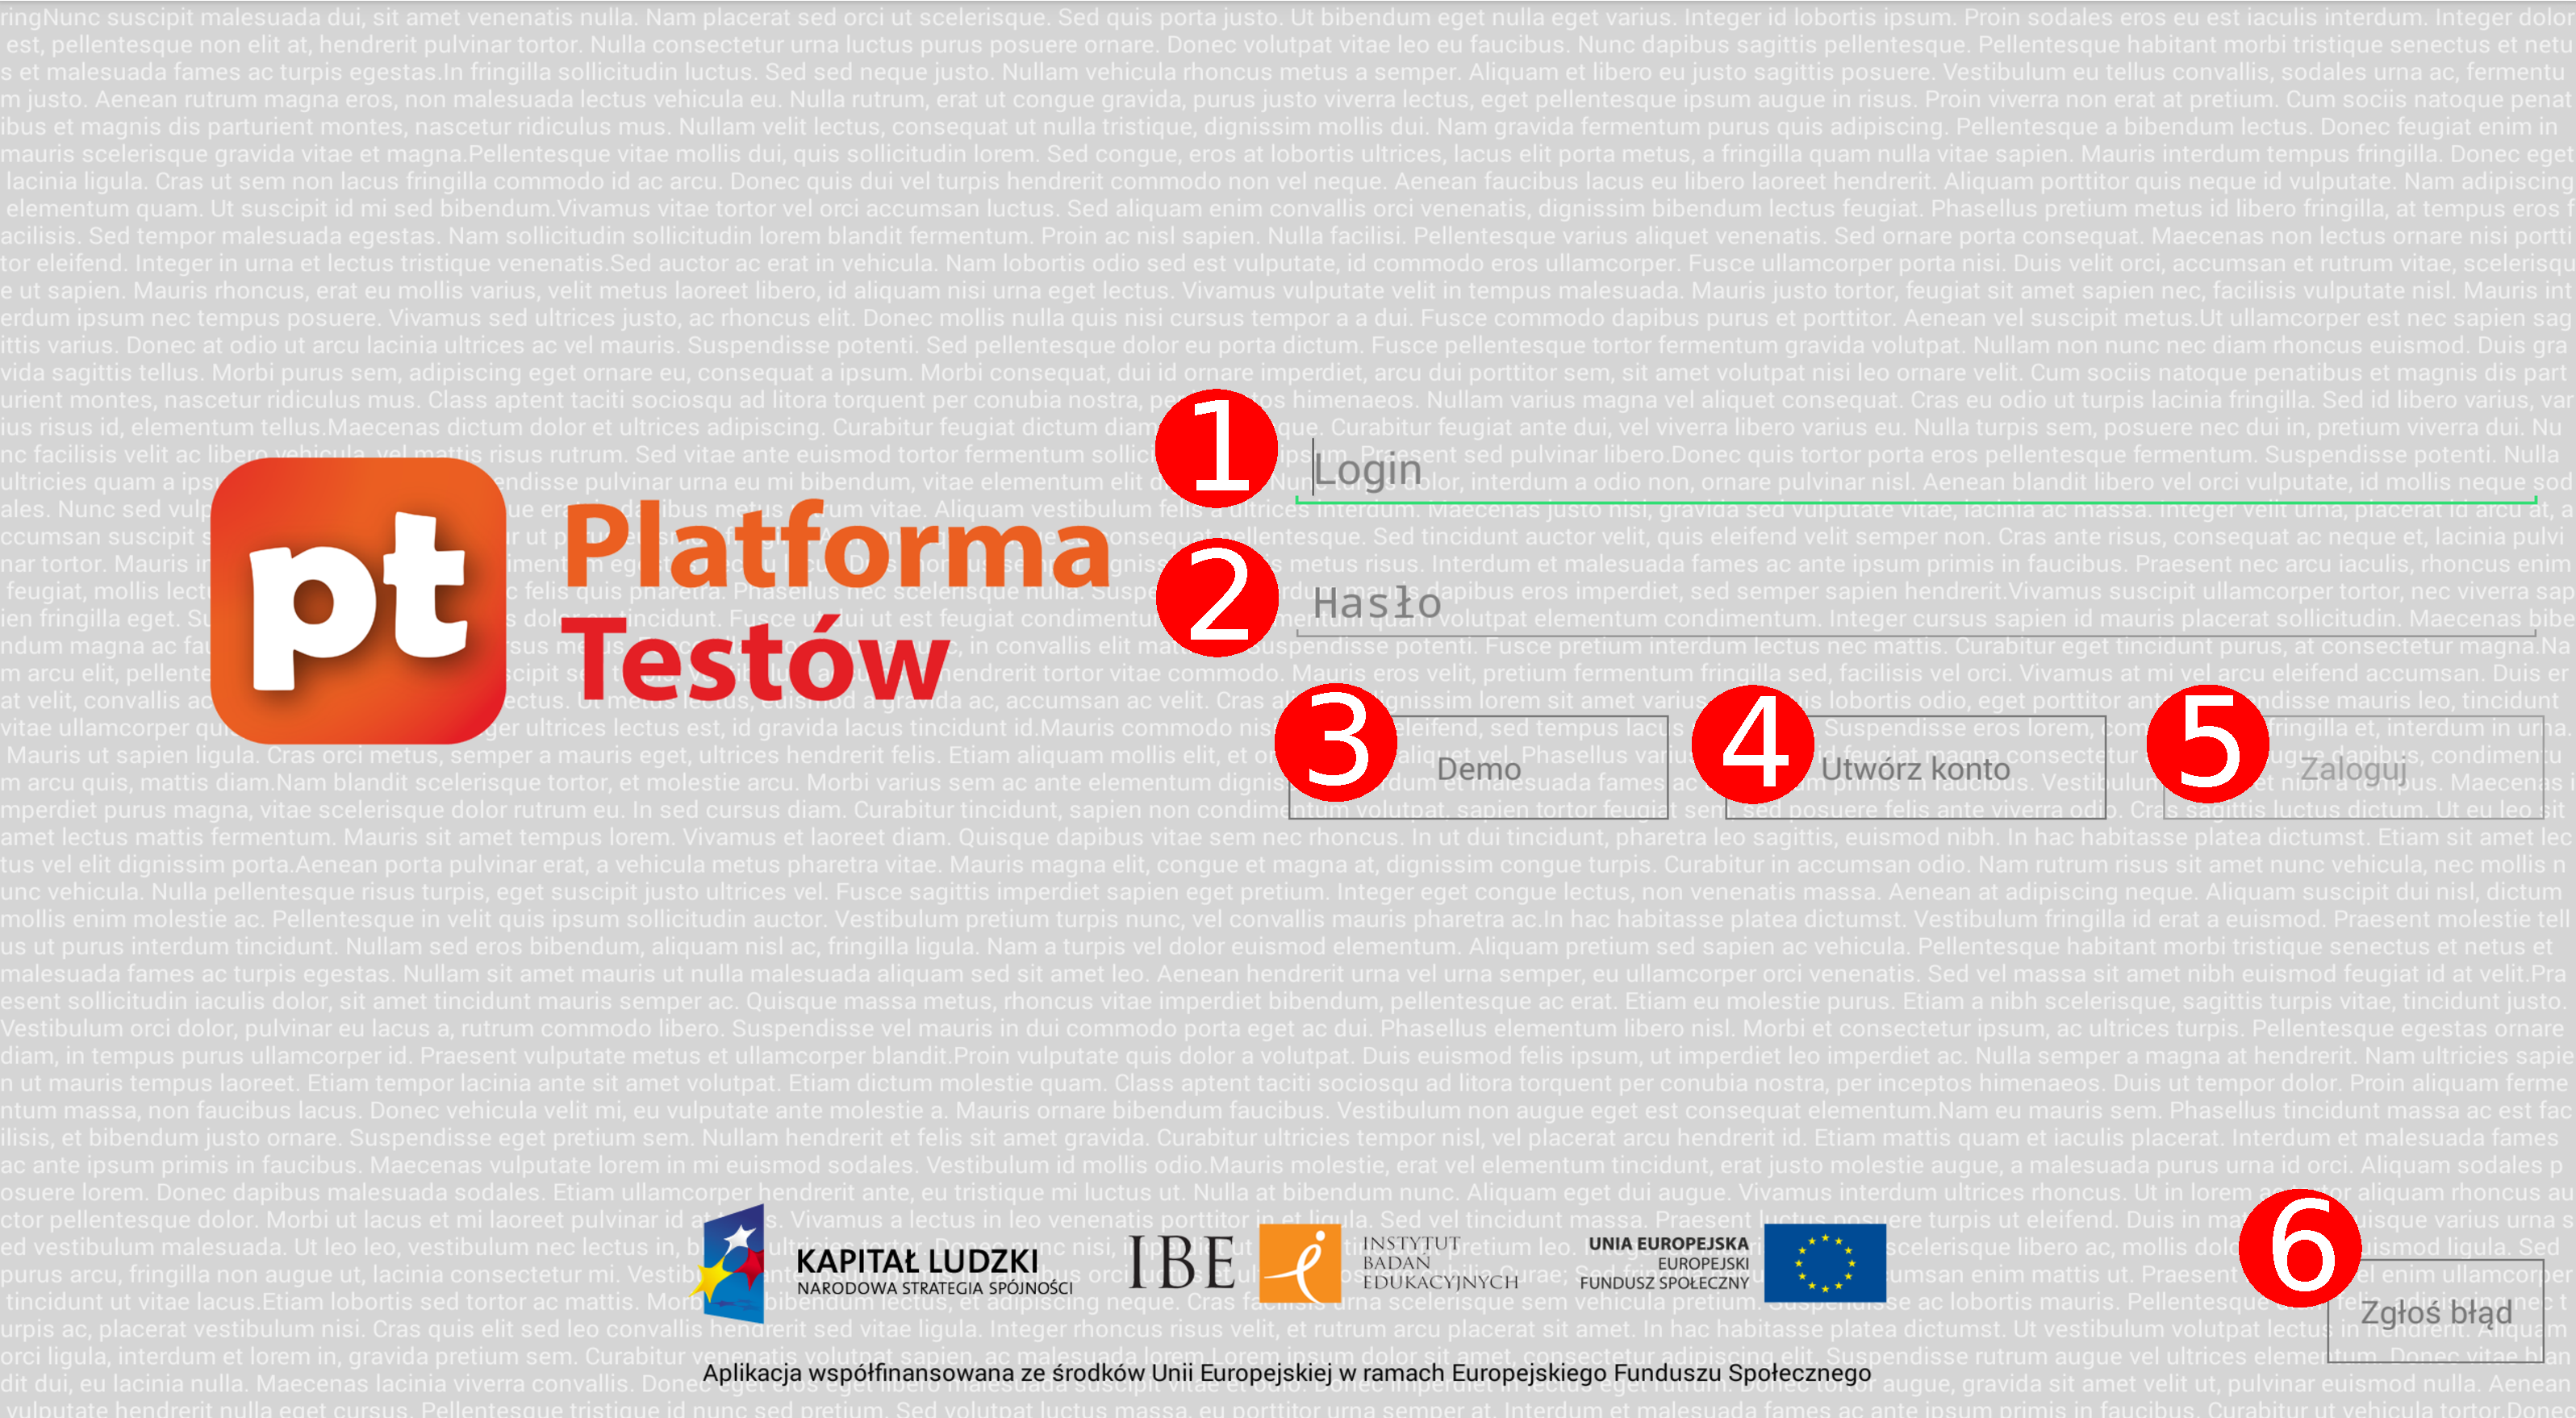
\includegraphics[width=0.95\textwidth]{activity_login.pdf}
\caption{Ekran logowania aplikacji}
\label{fig:login}
\end{figure}


\section{Operacje dostępne bez logowania}

Niezalogowany użytkownik ma dostęp do następujących operacji (numeracja z rysunku \pref{fig:login}):

\begin{itemize}
\item Uruchamianie trybu demonstracyjnego (przycisk 3)
\item Tworzenie nowego konta (przycisk 4)
\item Logowanie na istniejące konto (pola 1 i 2; przycisk 5)
\item Zgłaszanie błędów (przycisk 6)
\end{itemize}

Wszystkie powyższe operacje dostępne są na ekranie logowania. Szczegóły ich działania, oprócz procesu zgłaszania błędów, opisane są w niniejszym rozdziale. Proces zgłaszania błędów opisano w rozdziale \pref{chap:bug_report}.


\section{Tryb demonstracyjny}
\label{sec:login_demo}

Tryb demonstracyjny jest szczególnym trybem, łączącym w sobie wykonywanie testu oraz prezentację raportu. Nie jest on przeznaczony do przeprowadzania właściwych badań, a jedynie do prezentacji sposobu ich przeprowadzania, oraz wyglądu raportów generowanych przez aplikację.

W jednym urządzeniu może zostać zainstalowanych wiele pakietów demonstracyjnych jednocześnie. Wraz z aplikacją dostarczane są dwa takie pakiety, prezentujące możliwości aplikacji. Są one w istocie identyczne, różnią się wyłącznie używanym językiem - jeden z nich zawiera treści oraz wypowiedzi lektora w języku polskim, drugi w języku angielskim.

Oprócz pakietów dostarczonych wraz z aplikacją, każdy zainstalowany w aplikacji bank zadań może (ale nie musi) dostarczyć związany ze sobą pakiet demonstracyjny. Pakiety te traktowane są równorzędnie z pakietami dostarczonymi wraz z aplikacją.

\begin{wrapfigure}{l}{0.5\textwidth}
\vspace{-1em}
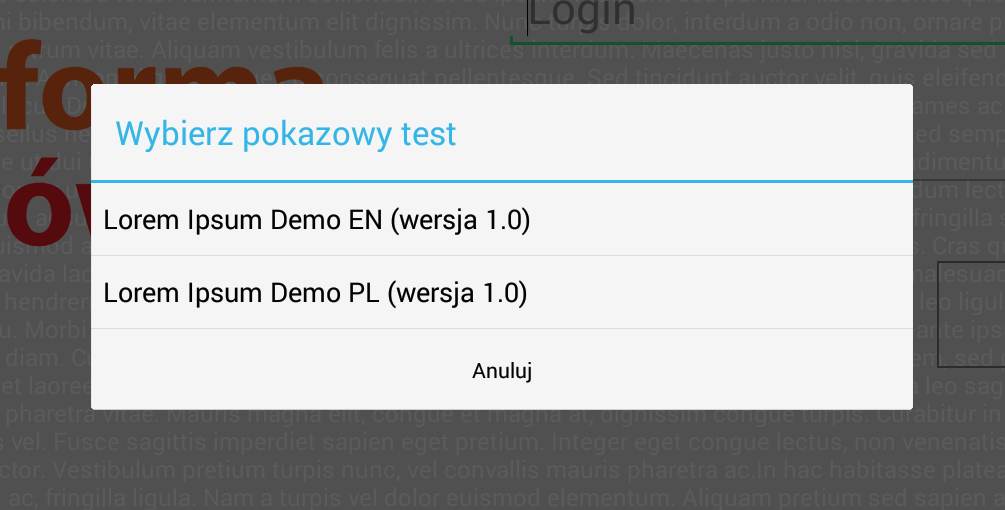
\includegraphics[width=0.48\textwidth]{activity_login-demos_list.png}
\caption{Lista pakietów demonstracyjnych, zawierająca wyłącznie dwa pakiety wbudowane w aplikację}
\label{fig:login_demo_list}
\end{wrapfigure}

Po wybraniu przycisku uruchamiającego tryb demonstracyjny (rysunek \ppref{fig:login}, przycisk 3) na ekranie logowania, wyświetlona zostaje lista zainstalowanych w urządzeniu pakietów demonstracyjnych (rysunek \ppref{fig:login_demo_list}).

Wybranie jednego z elementów listy skutkuje jego uruchomieniem. W pierwszej fazie, wyświetlane są kolejne zadania testowe. Nie jest tu jednak wykorzystywany algorytm CAT, ani nie jest wykonywane zbieranie wyników. Zadania wyświetlane są po kolei, a po ich zakończeniu następuje automatyczne przejście do demonstracyjnego raportu.

Więcej informacji na temat działania testu w trybie demonstracyjnym znajduje się w rozdziale \pref{sec:test_pilotdemotutorial_demo}. Informacje na temat działania raportu w trybie demonstracyjnym znajdują się w rozdziale \pref{sec:report_demo}.


\section{Proces tworzenia nowego konta}
\label{sec:login_createaccount}

\begin{wrapfigure}{r}{0.5\textwidth}
\vspace{-1em}
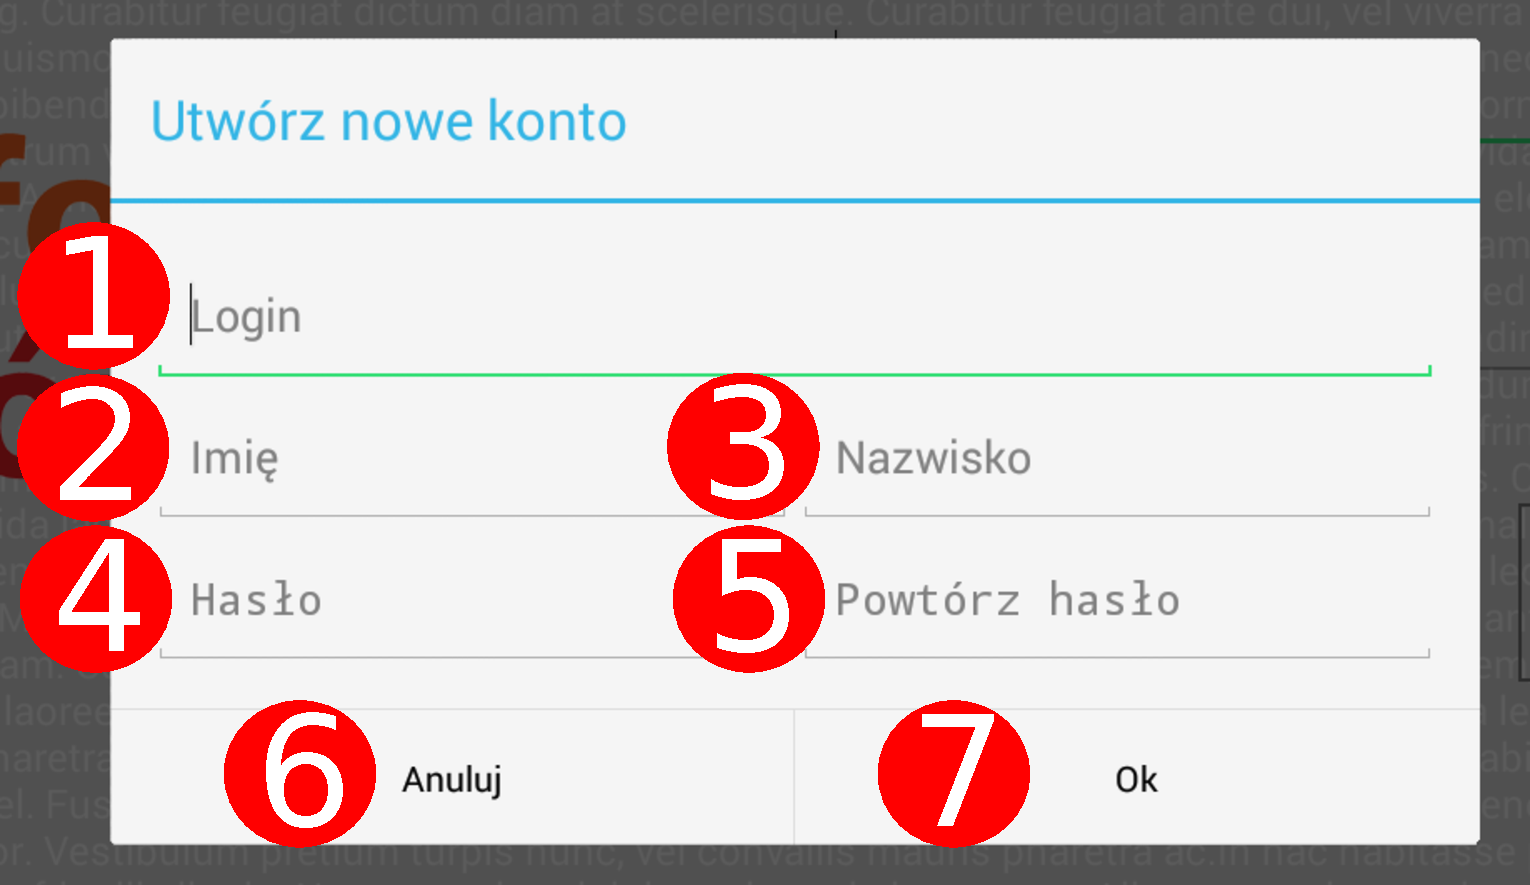
\includegraphics[width=0.48\textwidth]{activity_login-create_account.pdf}
\caption{Okno tworzenia nowego konta}
\label{fig:login_new_account}
\end{wrapfigure}

Aby móc się zalogować w aplikacji, wymagane jest posiadanie w niej własnego konta badacza. Konto badacza służy rozróżnieniu poszczególnych osób korzystających z aplikacji poprzez umożliwienie im korzystania z indywidualnie zainstalowanych banków zadań, wykonywanie testów na przypisanych do siebie badanych oraz przeglądanie utworzonych dla nich raportów.

Konto badacza tworzone jest przy użyciu przycisku tworzenia nowego konta na ekranie logowania (rysunek \ppref{fig:login}, przycisk 4). Wybranie tego przycisku powoduje wyświetlenie okna umożliwiającego utworzenie nowego konta.

Okno tworzenia konta widoczne jest na rysunku \pref{fig:login_new_account}. Rejestrujący się użytkownik powinien wpisać w widoczne pola następujące dane:

Pole nazwy użytkownika (1): nazwa użytkownika (login) której użytkownik będzie używał do identyfikacji w aplikacji. Musi ona zawierać co najmniej 6 znaków.

Pole imienia użytkownika (2): prawdziwe imię użytkownika.

Pole nazwiska użytkownika (3): prawdziwe nazwisko użytkownika.

Pole hasła (4): hasło, którego będzie używał użytkownik w celu uzyskania dostępu do swojego konta w aplikacji. Hasło powinno być odpowiednio skomplikowane by zapewnić bezpieczeństwo i nie powinno być przekazywane innym osobom. Musi zawierać co najmniej 6 znaków.

Pole powtórzenia hasła (5): to samo hasło, które zostało wpisane w polu hasła (4). Dwukrotne wpisanie hasła upewnia aplikację że w treści hasła nie doszło do przypadkowego błędu.

Po zakończeniu wypełniania pól, należy nacisnąć przycisk \emph{OK} (7). Konto zostanie utworzone, a aplikacja przeniesie użytkownika wprost do ekranu wyboru banku zadań (rozdział \ppref{chap:suiteselect}).

W celu wyjścia z okna bez tworzenia nowego konta, należy nacisnąć przycisk \emph{Anuluj} (6).


\section{Proces logowania}

Do zalogowania w aplikacji wymagane jest posiadanie w niej konta. Proces jego rejestracji opisany jest w rozdziale \pref{sec:login_createaccount}.

W celu zalogowania do aplikacji należy wpisać następujące dane: nazwę użytkownika (login) w pole \emph{Login} (rysunek \ppref{fig:login}, pole 1), oraz hasło w pole \emph{Hasło} (rysunek \ppref{fig:login}, pole 2). Muszą być to poprawne dane uprzednio zarejestrowanego konta. 

Po wpisaniu danych należy nacisnąć przycisk \emph{Zaloguj} (rysunek \ppref{fig:login}, przycisk 5). Proszę zwrócić uwagę, że nie jest możliwe wciśnięcie przycisku bez uprzedniego wpisania co najmniej 6 znaków w obydwa pola.

Jeżeli wpisane zostały poprawne dane, użytkownik przeniesiony zostanie do ekranu wyboru banku zadań (rozdział \ppref{chap:suiteselect}). W przeciwnym wypadku, wyświetlony zostanie komunikat o niepowodzeniu.


\chapter{Ekran wyboru banku zadań}
\label{chap:suiteselect}

\begin{figure}[b!]
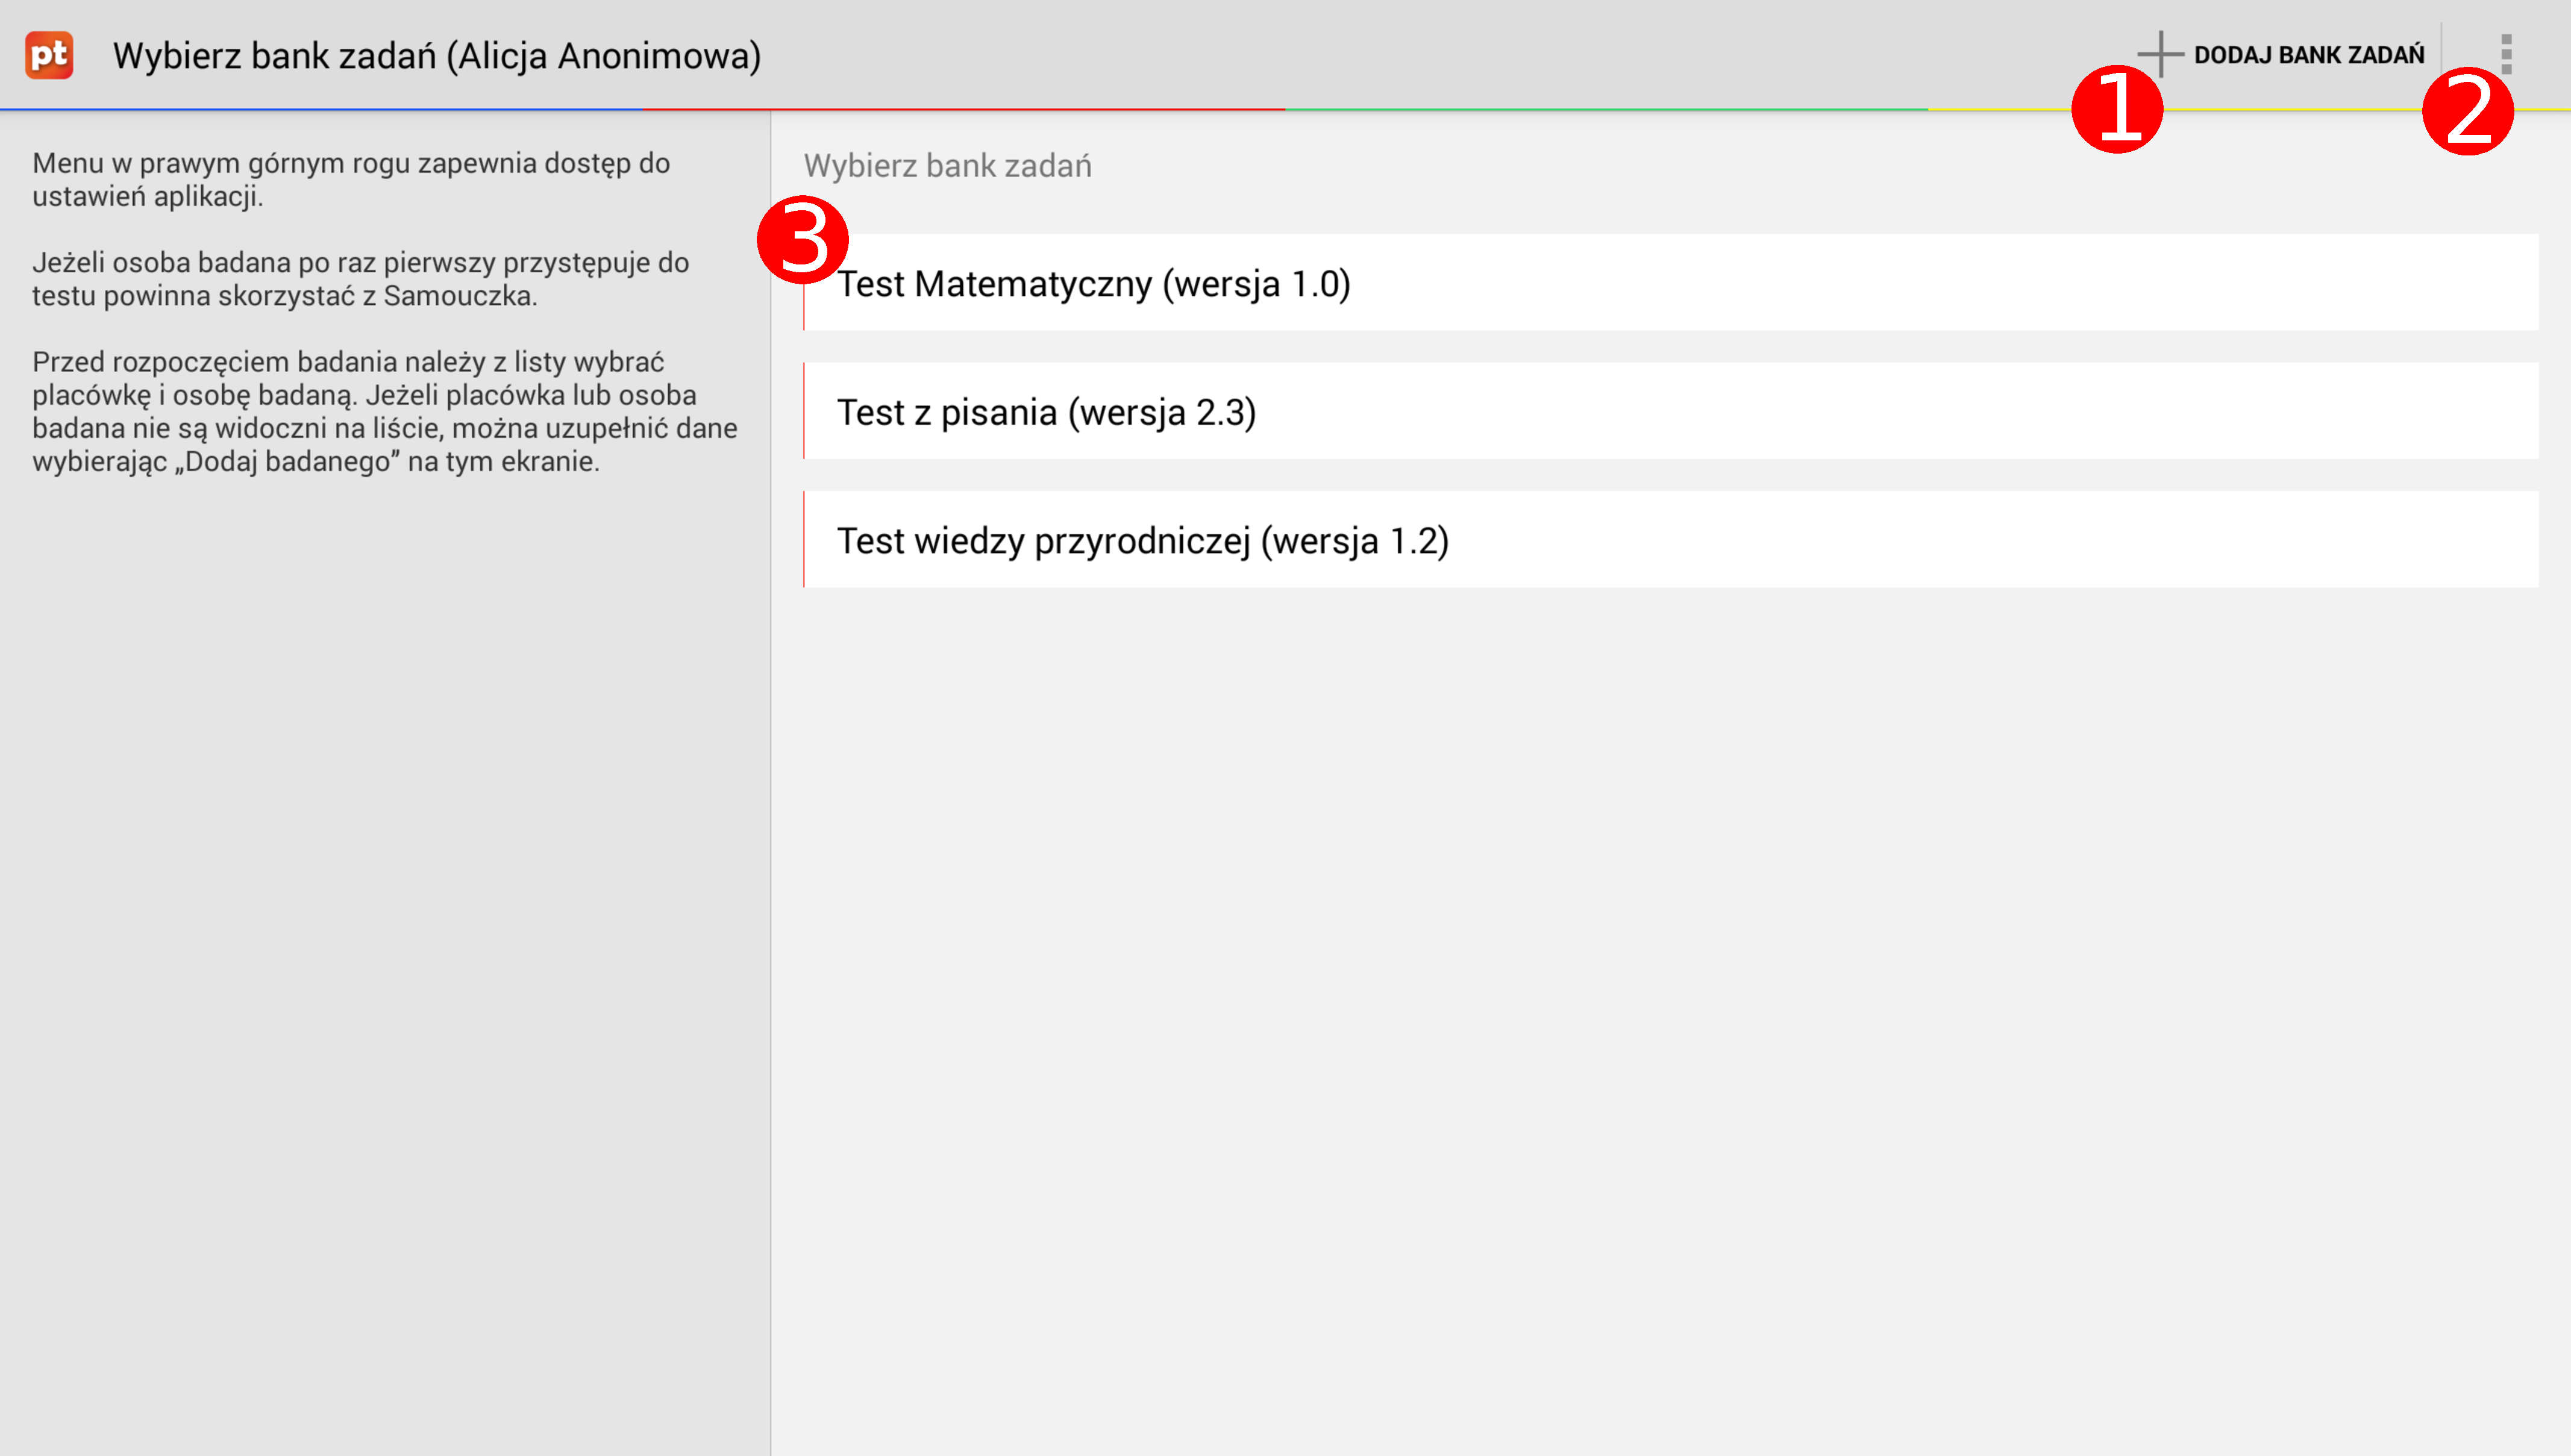
\includegraphics[width=0.96\textwidth]{activity_suite_select.pdf}
\caption{Ekran wyboru banku zadań}
\label{fig:suiteselect}
\end{figure}

Ekran wyboru banków zadań służy do wybrania banku, z którego chce korzystać użytkownik (rysunek \ppref{fig:suiteselect}). Wybór następuje poprzez naciśniecie jednego z elementów listy (3). Po jego wybraniu, bank zadań jest ładowany, a następnie wyświetlany jest główny ekran aplikacji (rozdział \ppref{chap:main}).

Oprócz wyboru jednego z aktualnie zainstalowanych banków zadań, możliwe jest dodanie kolejnych (przycisk 1). Opis znajduje się w kolejnym rozdziale (rozdział \ppref{sec:suiteselect_add}). Oprócz tego, możliwe jest wywołanie menu przy pomocy przycisku w prawym górnym rogu ekranu (2). Menu dostarcza opcję zgłaszania błędu, która opisana jest w rozdziale \pref{chap:bug_report}.

Naciśnięcie i dłuższe przytrzymanie jednego z banków zadań spowoduje pokazanie dodatkowego menu, umożliwiającego m.in. odinstalowanie banku zadań. 

\section{Dodawanie banków zadań}
\label{sec:suiteselect_add}

\begin{wrapfigure}{r}{0.5\textwidth}
\vspace{-1em}
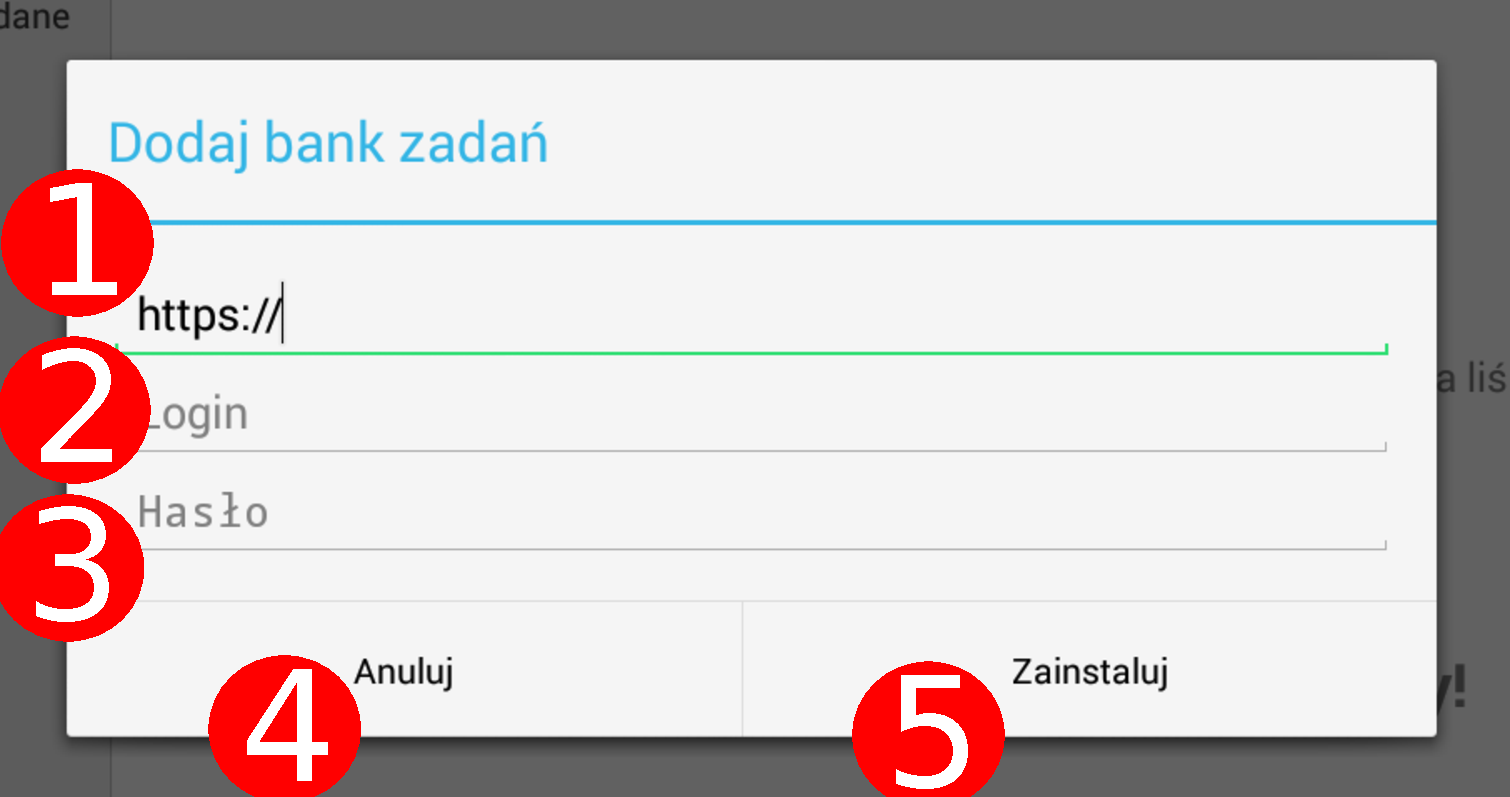
\includegraphics[width=0.48\textwidth]{activity_suite_select-add_task_suite.pdf}
\caption{Okno dodawania banku zadań}
\vspace{-1em}
\label{fig:suiteselect_add}
\end{wrapfigure}

W celu dodania nowego banku zadań, należy nacisnąć przycisk dodawania nowego banku (rysunek \ppref{fig:suiteselect}, przycisk 1). Po jego wybraniu wyświetlone zostanie okno dodawania banku zadań (rysunek \ppref{fig:suiteselect_add}).

Pola w oknie należy wypełnić w następujący sposób:

W pole adresu sieciowego (1) należy wpisać adres internetowy pod którym dostępny jest bank zadań. Adres ten powinien zostać przekazany przez autorów lub osoby odpowiedzialne za publikację banku zadań.

W pole nazwy użytkownika (loginu; 2) należy wpisać swoją nazwę użytkownika na serwerze dostarczającym bank zadań. Zazwyczaj \emph{nie} jest to ta sama nazwa której używa użytkownik do zalogowania w aplikacji.

W pole hasła (3) należy wpisać hasło do serwera banku zadań, skojarzone z podaną wcześniej nazwą użytkownika. Zazwyczaj \emph{nie} jest to to samo hasło którego używa użytkownik do zalogowania w aplikacji.

\begin{wrapfigure}{l}{0.5\textwidth}
\vspace{-1em}
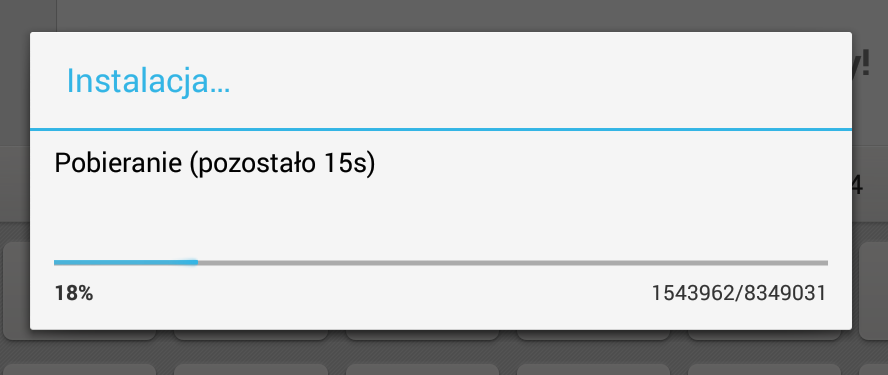
\includegraphics[width=0.48\textwidth]{activity_suite_select-installing.png}
\caption{Okno informujące o pobieraniu banku zadań}
\vspace{-1em}
\label{fig:suiteselect_installation}
\end{wrapfigure}

W celu uruchomienia instalacji, należy nacisnąć przycisk ``Zainstaluj"\hspace{1em}(5). Uruchomione zostanie pobieranie banku zadań z podanego adresu. 

Podczas pobierania na ekranie widoczne jest okno jak na rysunku \pref{fig:suiteselect_installation}. Nie należy przerywać procedury pobierania banku zadań, inaczej konieczne będzie przeprowadzenie jej ponownie.
Po zakończeniu procesu, na liście pojawi się nowy bank zadań. Wybranie go spowoduje przejście do okna głównego aplikacji.

\begin{wrapfigure}{r}{0.5\textwidth}
%\vspace{-1em}
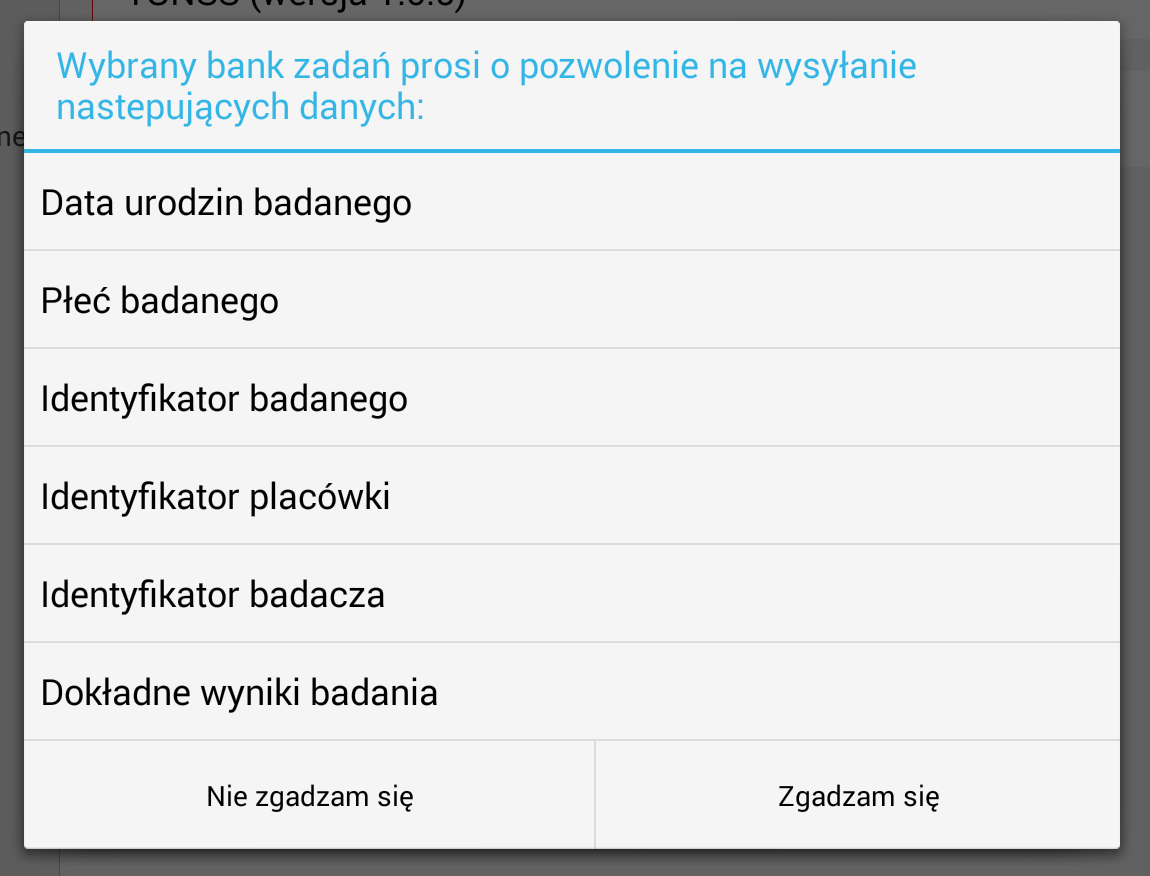
\includegraphics[width=0.48\textwidth]{activity_suite_select-result_submit_approval_request.png}
\caption{Okno decyzji dotyczącej wysyłania zanonimizowanych wyników}
\vspace{-1em}
\label{fig:suiteselect_sendresults}
\end{wrapfigure}

\vspace{1em}
Jeżeli bank zadań zbiera wyniki i przesyła je do operatora, to podczas pierwszego uruchamiania wyświetlone zostanie zapytanie o zgodę na ich wysyłanie (rysunek \ppref{fig:suiteselect_sendresults}). Po naciśnięciu dowolnego z widocznych wówczas przycisków, użytkownik zostaje przeniesiony do głównego ekranu aplikacji. Decyzję odnośnie wysyłania wyników można zawsze zmienić w ustawieniach (rozdział \ppref{sec:main_settings}).

\chapter{Ekran główny aplikacji}
\label{chap:main}

Ekran główny aplikacji jest centralnym miejscem, z którego użytkownik uzyskuje dostęp do większości funkcji aplikacji.

\begin{figure}[b!]
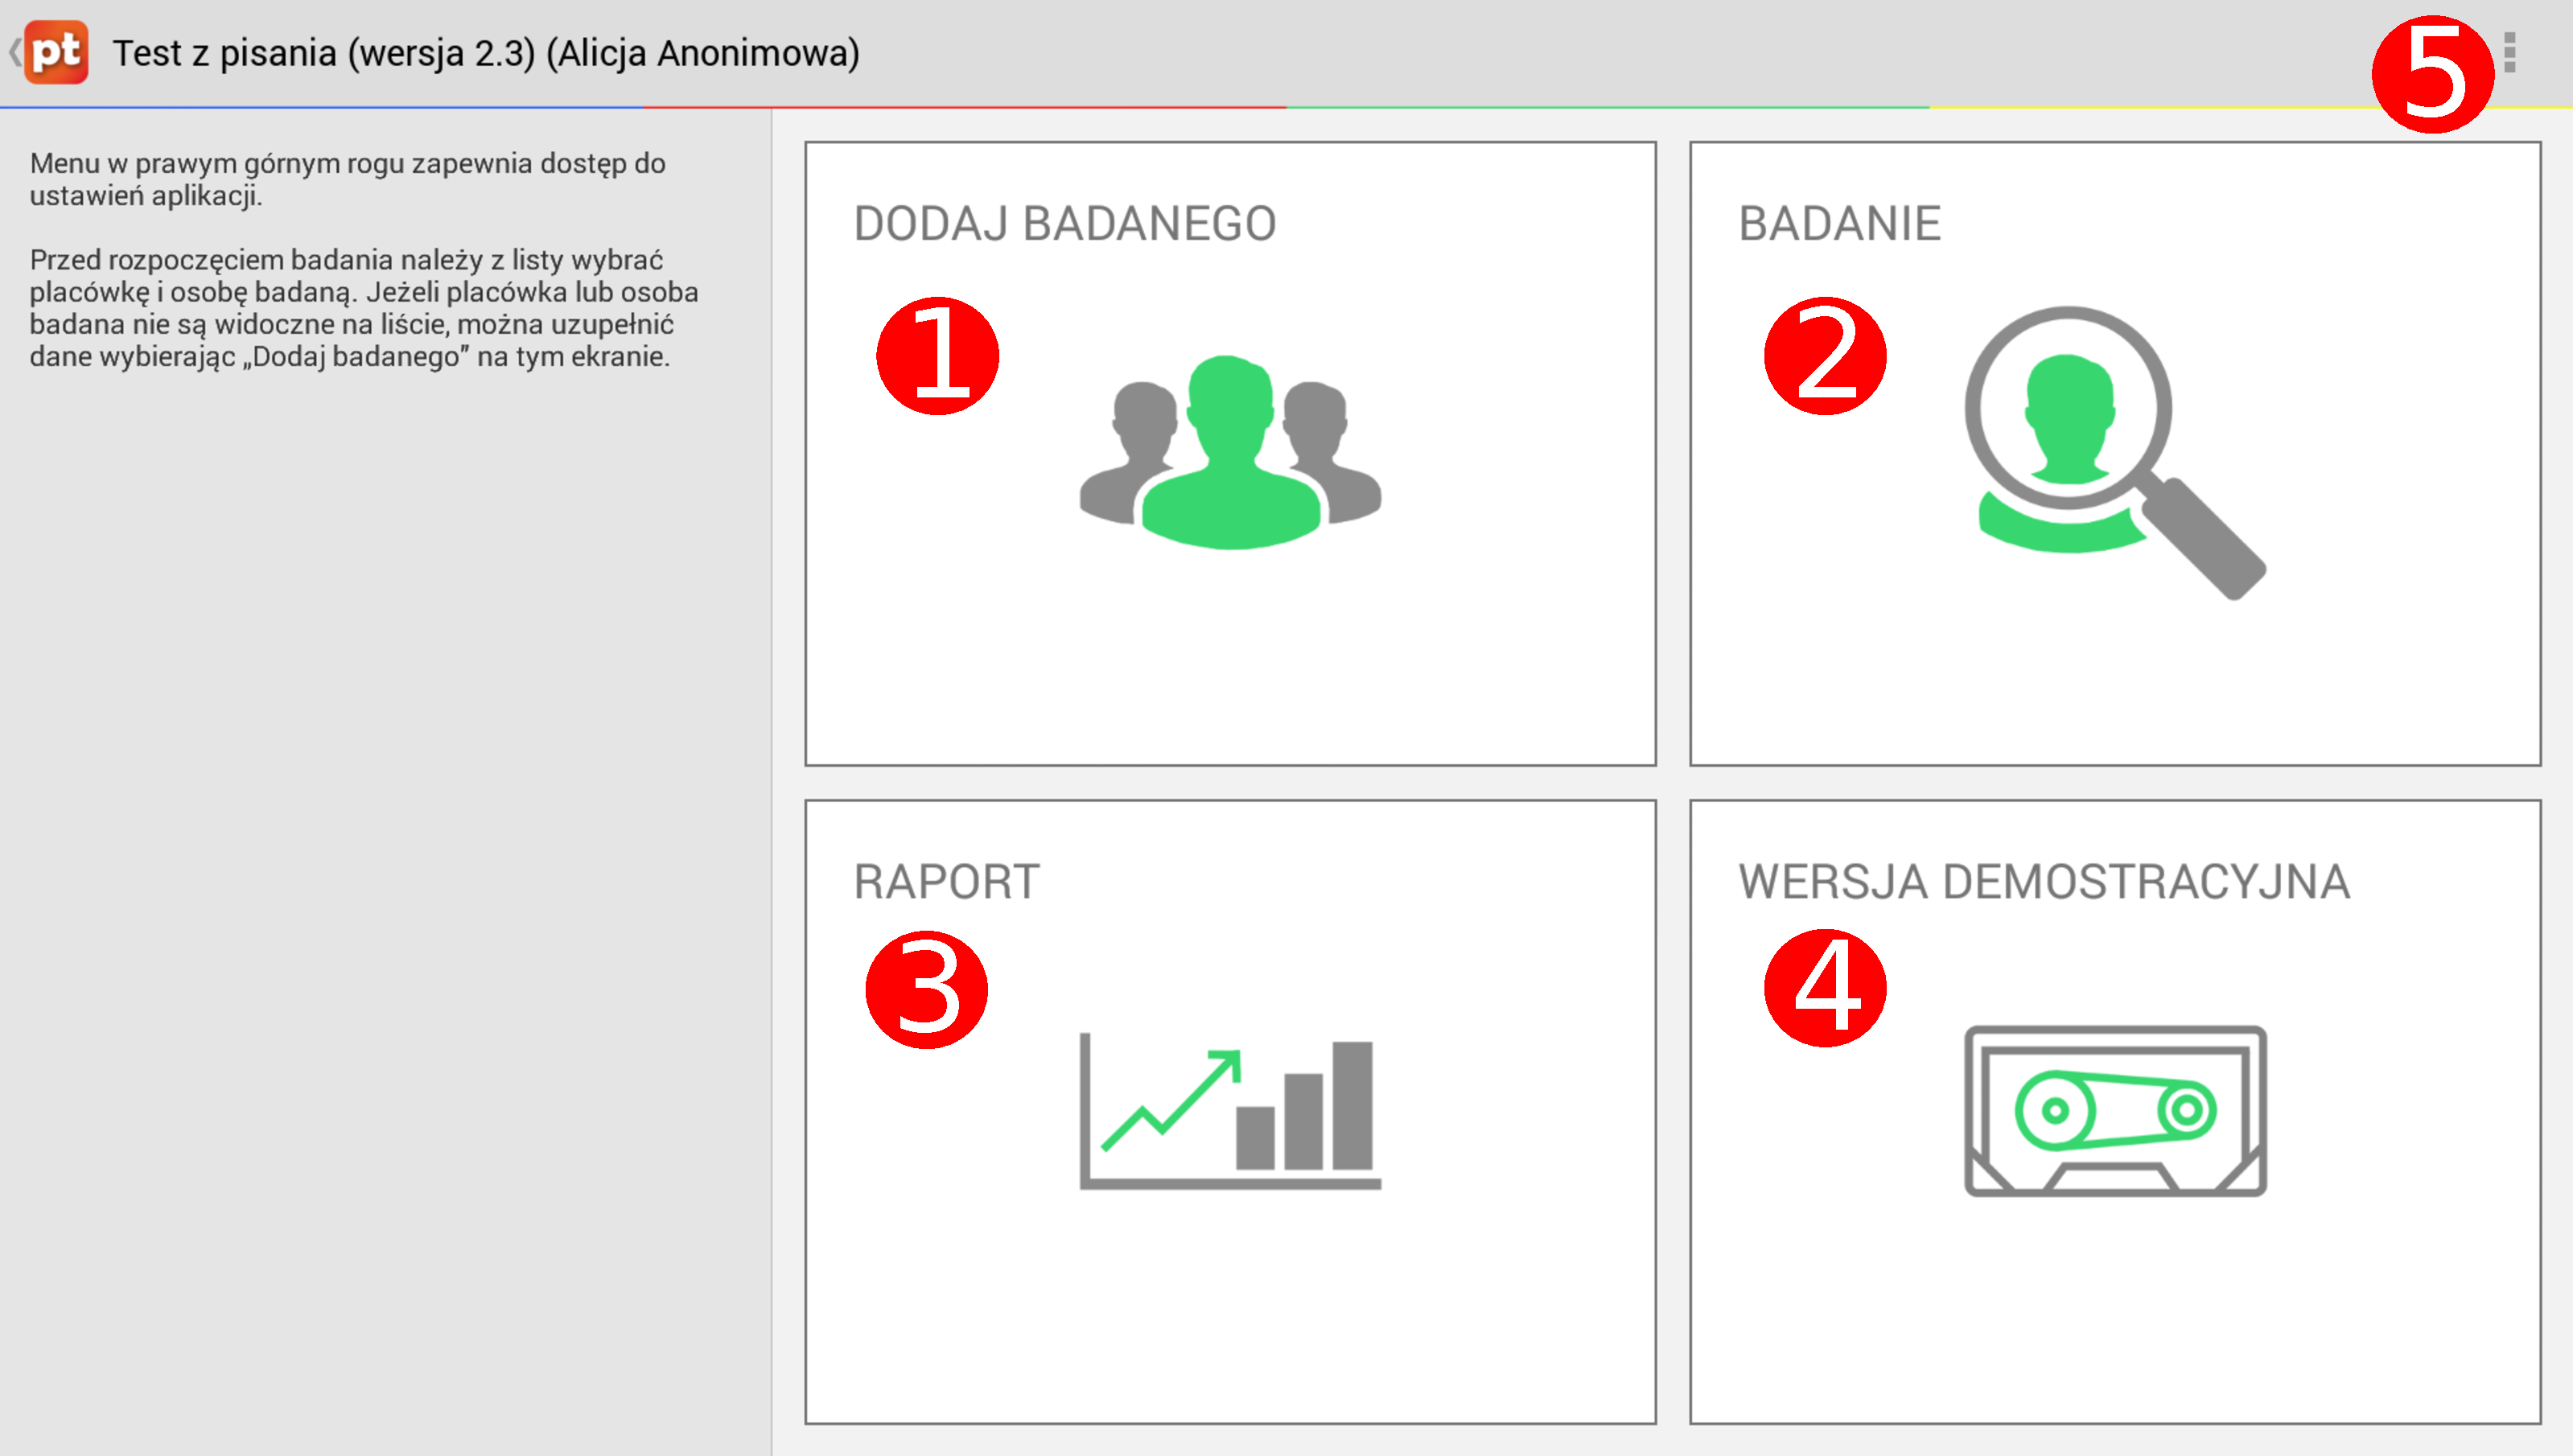
\includegraphics[width=0.96\textwidth]{activity_main.pdf}
\caption{Ekran główny aplikacji}
\label{fig:main}
\end{figure}

Przy pomocy przycisków na ekranie głównym użytkownik przemieszcza się pomiędzy pozostałymi ekranami aplikacji (rysunek \pref{fig:main}).

Przycisk dodawania badanego (1) przenosi do ekranu dodawania badanych (rozdział \ppref{chap:examineemgr}).

Przycisk rozpoczęcia badania (2) przenosi do ekranu uruchamiania testu (rozdział \ppref{chap:runtest}). Aby rozpocząć test, konieczne jest włączenie w urządzeniu \emph{trybu samolotowego} (na niektórych urządzeniach określanego jako \emph{tryb offline}). W przypadku gdy tryb samolotowy jest nieaktywny w momencie rozpoczynania badania, wyświetlony zostaje komunikat jak na rysunku \pref{fig:main_airplanemode}. Wybranie przycisku ``Ok'' przeniesie użytkownika do odpowiedniego ekranu w ustawieniach systemu, gdzie możliwe będzie aktywowanie trybu samolotowego. Po zaznaczeniu tej opcji, użytkownik powinien użyć przycisku powrotu, aby powrócić do aplikacji.

\begin{wrapfigure}{r}{0.5\textwidth}
\vspace{-2em}
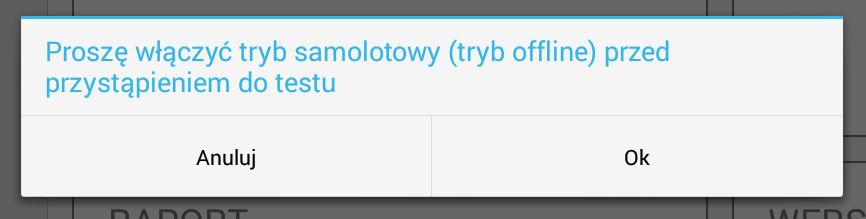
\includegraphics[width=0.48\textwidth]{activity_main-offline_mode.png}
\caption{Ostrzeżenie o nieaktywnym trybie samolotowym}
\label{fig:main_airplanemode}
\end{wrapfigure}

Przycisk raportu (3) przenosi do ekranu raportu (rozdział \ppref{chap:report}).

Przycisk wersji demonstracyjnej (4) powoduje uruchomienie trybu demonstracyjnego dla aktualnie uruchomionego banku zadań. W pierwszej fazie tego trybu, wyświetlane są kolejne zadania testowe. Nie jest tu jednak wykorzystywany algorytm CAT, ani nie jest wykonywane zbieranie wyników. Zadania wyświetlane są po kolei, a po ich zakończeniu następuje automatyczne przejście do demonstracyjnego raportu.

Więcej informacji na temat działania testu w trybie demonstracyjnym znajduje się w rozdziale \pref{sec:test_pilotdemotutorial_demo}. Informacje na temat działania raportu w trybie demonstracyjnym znajdują się w rozdziale \pref{sec:report_demo}.

\begin{wrapfigure}{r}{0.25\textwidth}
\vspace{-1em}
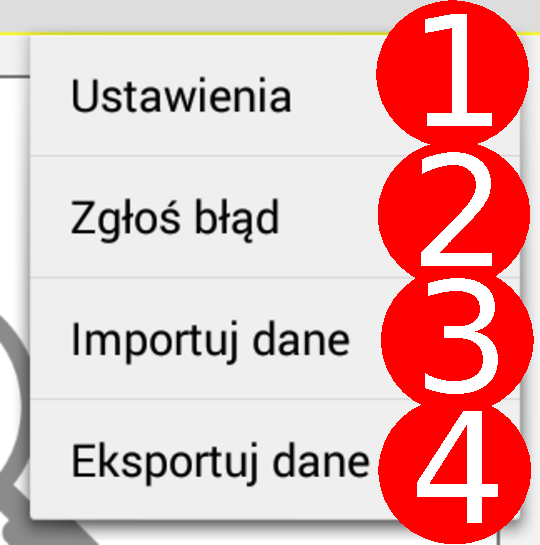
\includegraphics[width=0.24\textwidth]{activity_main-menu.pdf}
\caption{Wygląd menu ekranu głównego}
\label{fig:main_menu}
\end{wrapfigure}

Przycisk menu (5) powoduje rozwinięcie menu dla tego ekranu. Wygląd menu przedstawiono na rysunku \pref{fig:main_menu}. Daje ono dostęp do kilku dodatkowych funkcji:

Polecenie ``Ustawienia'' (1) powoduje otwarcie okna ustawień dla aktualnego banku zadań (rozdział \ppref{sec:main_settings}).

Polecenie ``Zgłoś błąd'' (2) powoduje otwarcie okna zgłaszania błędów w aplikacji (rozdział \ppref{chap:bug_report}).

Polecenie ``Importuj dane'' (3) powoduje wykonanie importu danych z karty SD do aplikacji.

Polecenie ``Eksportuj dane'' (4) powoduje wykonanie eksportu danych z aplikacji na kartę SD.


\section{Ustawienia}
\label{sec:main_settings}

\begin{figure}[h!]
\centering
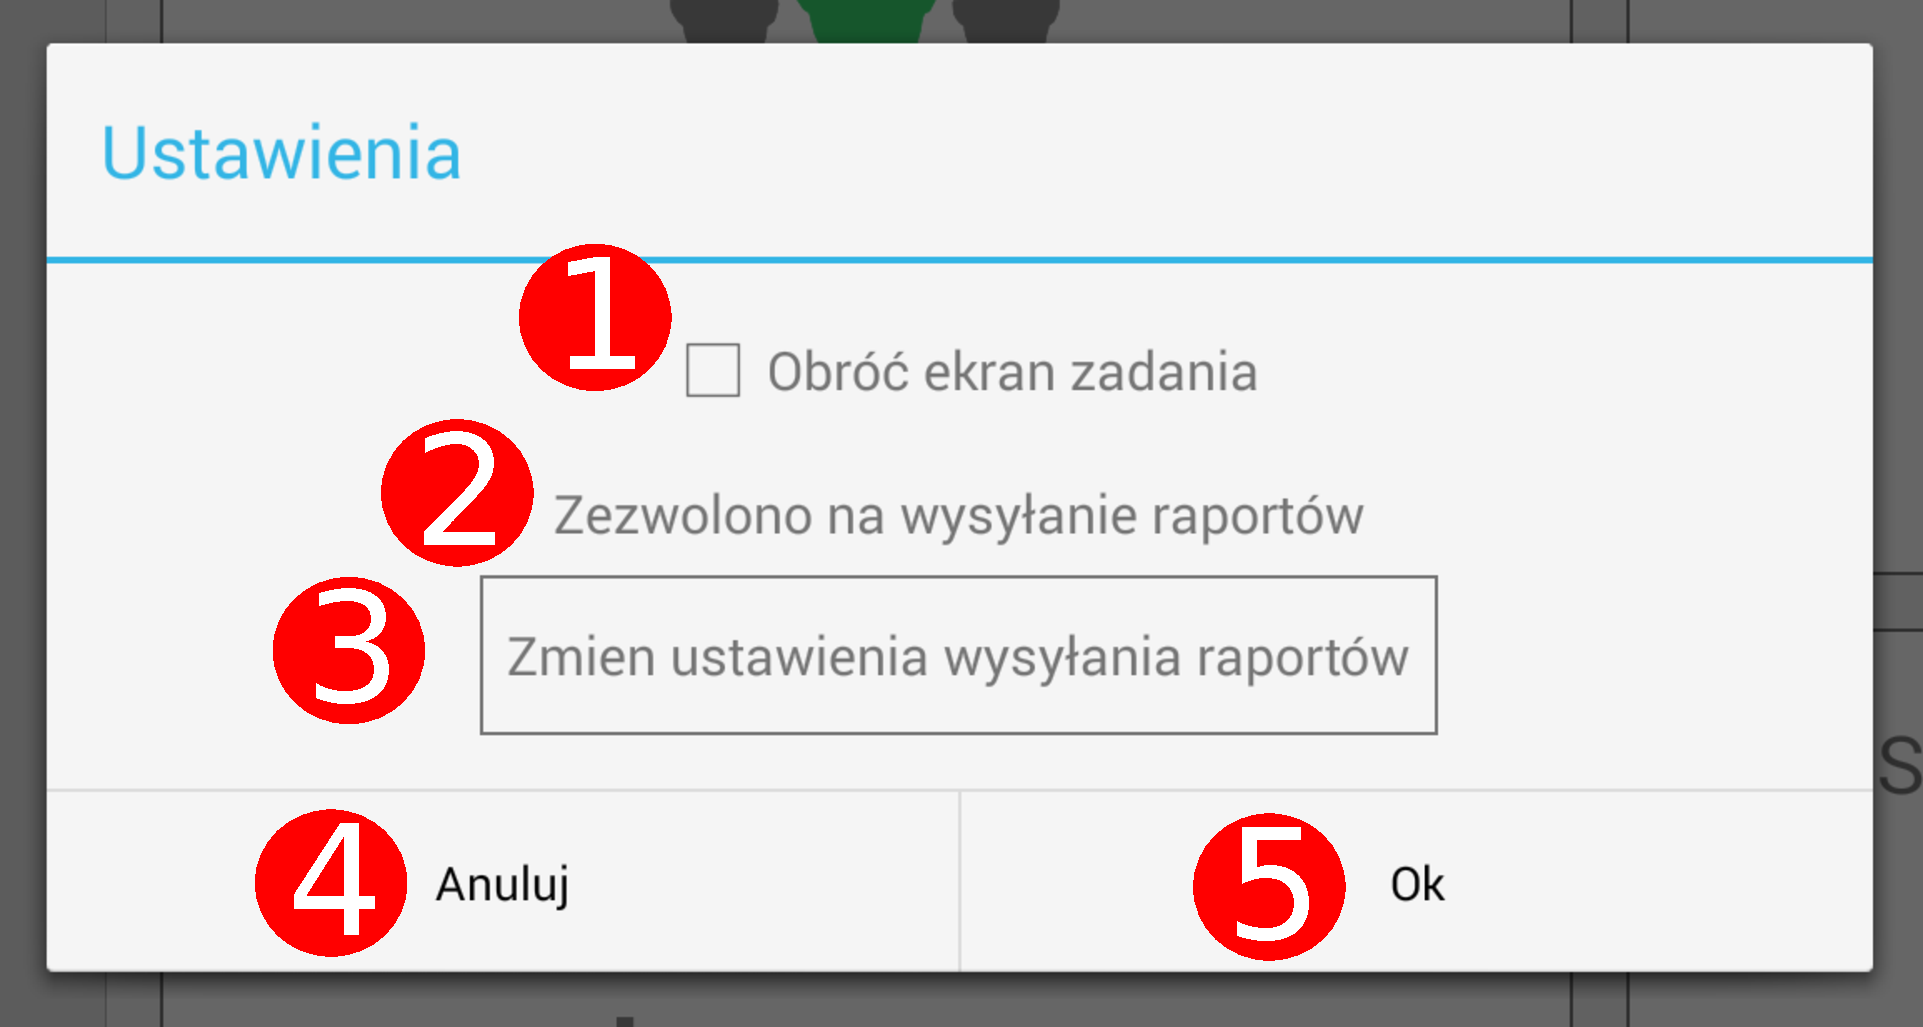
\includegraphics[width=0.48\textwidth]{activity_main-settings.pdf}
\caption{Okno ustawień banku zadań}
\label{fig:main_settings}
\end{figure}

Okno ustawień pozwala dostosować zachowanie banku zadań. W tym oknie znajdują się (rysunek \ppref{fig:main_settings}):

(1) Opcja pozwalająca zdecydować, czy zadanie na ekranie testu (rozdział \ppref{chap:test}) ma być wyświetlane tak jak reszta interfejsu użytkownika, czy w położeniu odwróconym o 180\textdegree. Opcja ta utrudnia osobie badanej przypadkowe naciśnięcie przycisków sterujących systemu Android które znajdują się na dole ekranu\footnote{Opisywany problem nie występuje w systemach Android w wersji 4.4 i nowszych. Na tych systemach aplikacja używa \emph{immersive mode} w którym przyciski sterujące nie są widoczne.}. Ustawienie to jest również użyteczne, gdy badacz i osoba badana znajdują się naprzeciwko siebie.

\begin{wrapfigure}{r}{0.5\textwidth}
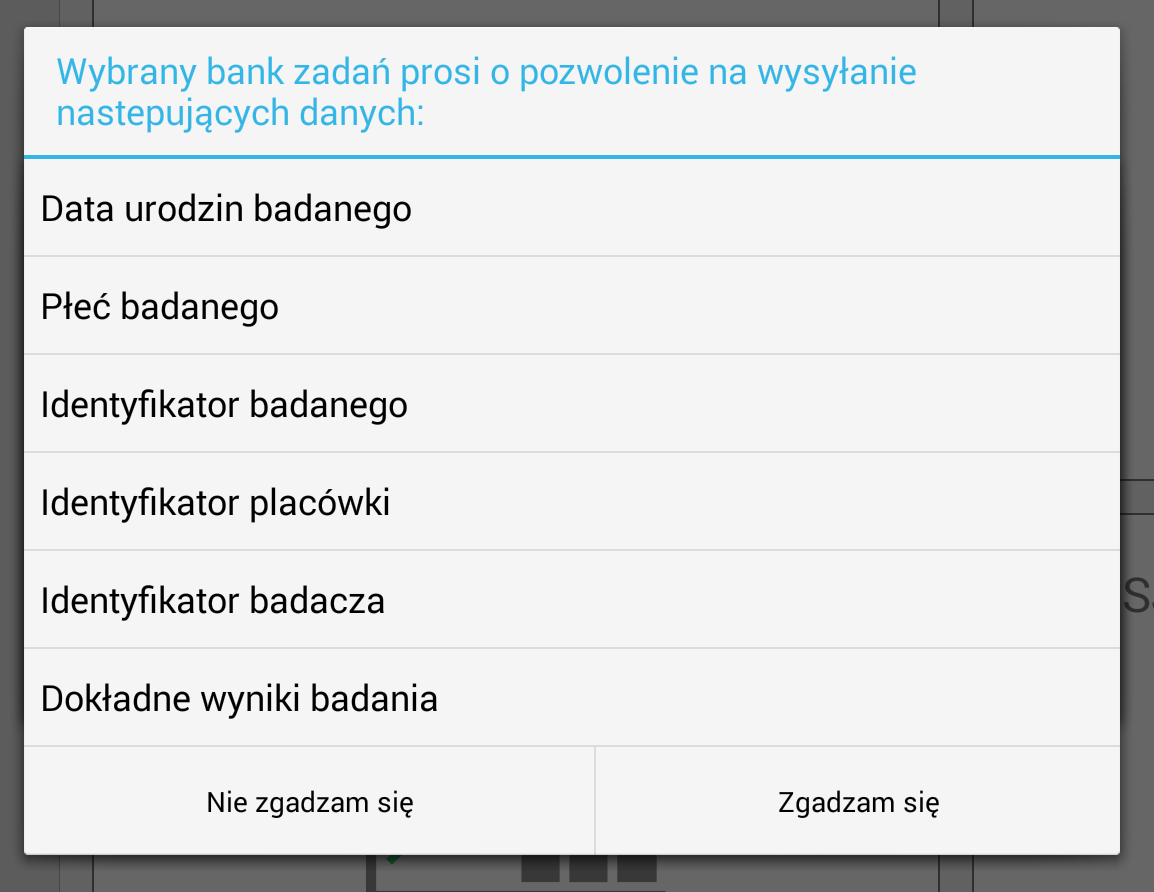
\includegraphics[width=0.48\textwidth]{activity_main-settings_result_submit_approval.png}
\caption{Okno decyzji dotyczącej wysyłania zanonimizowanych wyników}
\label{fig:main_settings_results}
\end{wrapfigure}

(2) Informacja o obecnym statusie zezwolenia na wysyłanie zanonimizowanych raportów do operatora banku zadań. Opcja ta jest początkowo ustawiana w oknie wyświetlanym podczas pierwszego uruchomienia banku zadań (rozdział \ppref{sec:suiteselect_add}), a następnie może być zmieniana za pomocą przycisku (3) poniżej.

(3) Przycisk pozwalający zmienić zezwolenie na wysyłanie zanonimizowanych raportów do operatora banku zadań. Aktualny status zezwolenia widoczny jest powyżej przycisku (2). Po wybraniu tej opcji wyświetlone zostanie okno (rysunek \ppref{fig:main_settings_results}) z informacją jakie dane będą wysyłane, oraz przyciskami pozwalającymi zezwolić bądź zabronić wysyłania.

(4) Przycisk ``Anuluj'' pozwala wyjść z ustawień bez ich zapisywania

(5) Przycisk ``Ok'' pozwala zapisać ustawienia i zamknąć okno

\chapter{Ekran dodawania badanych}
\label{chap:examineemgr}

\begin{figure}[b!]
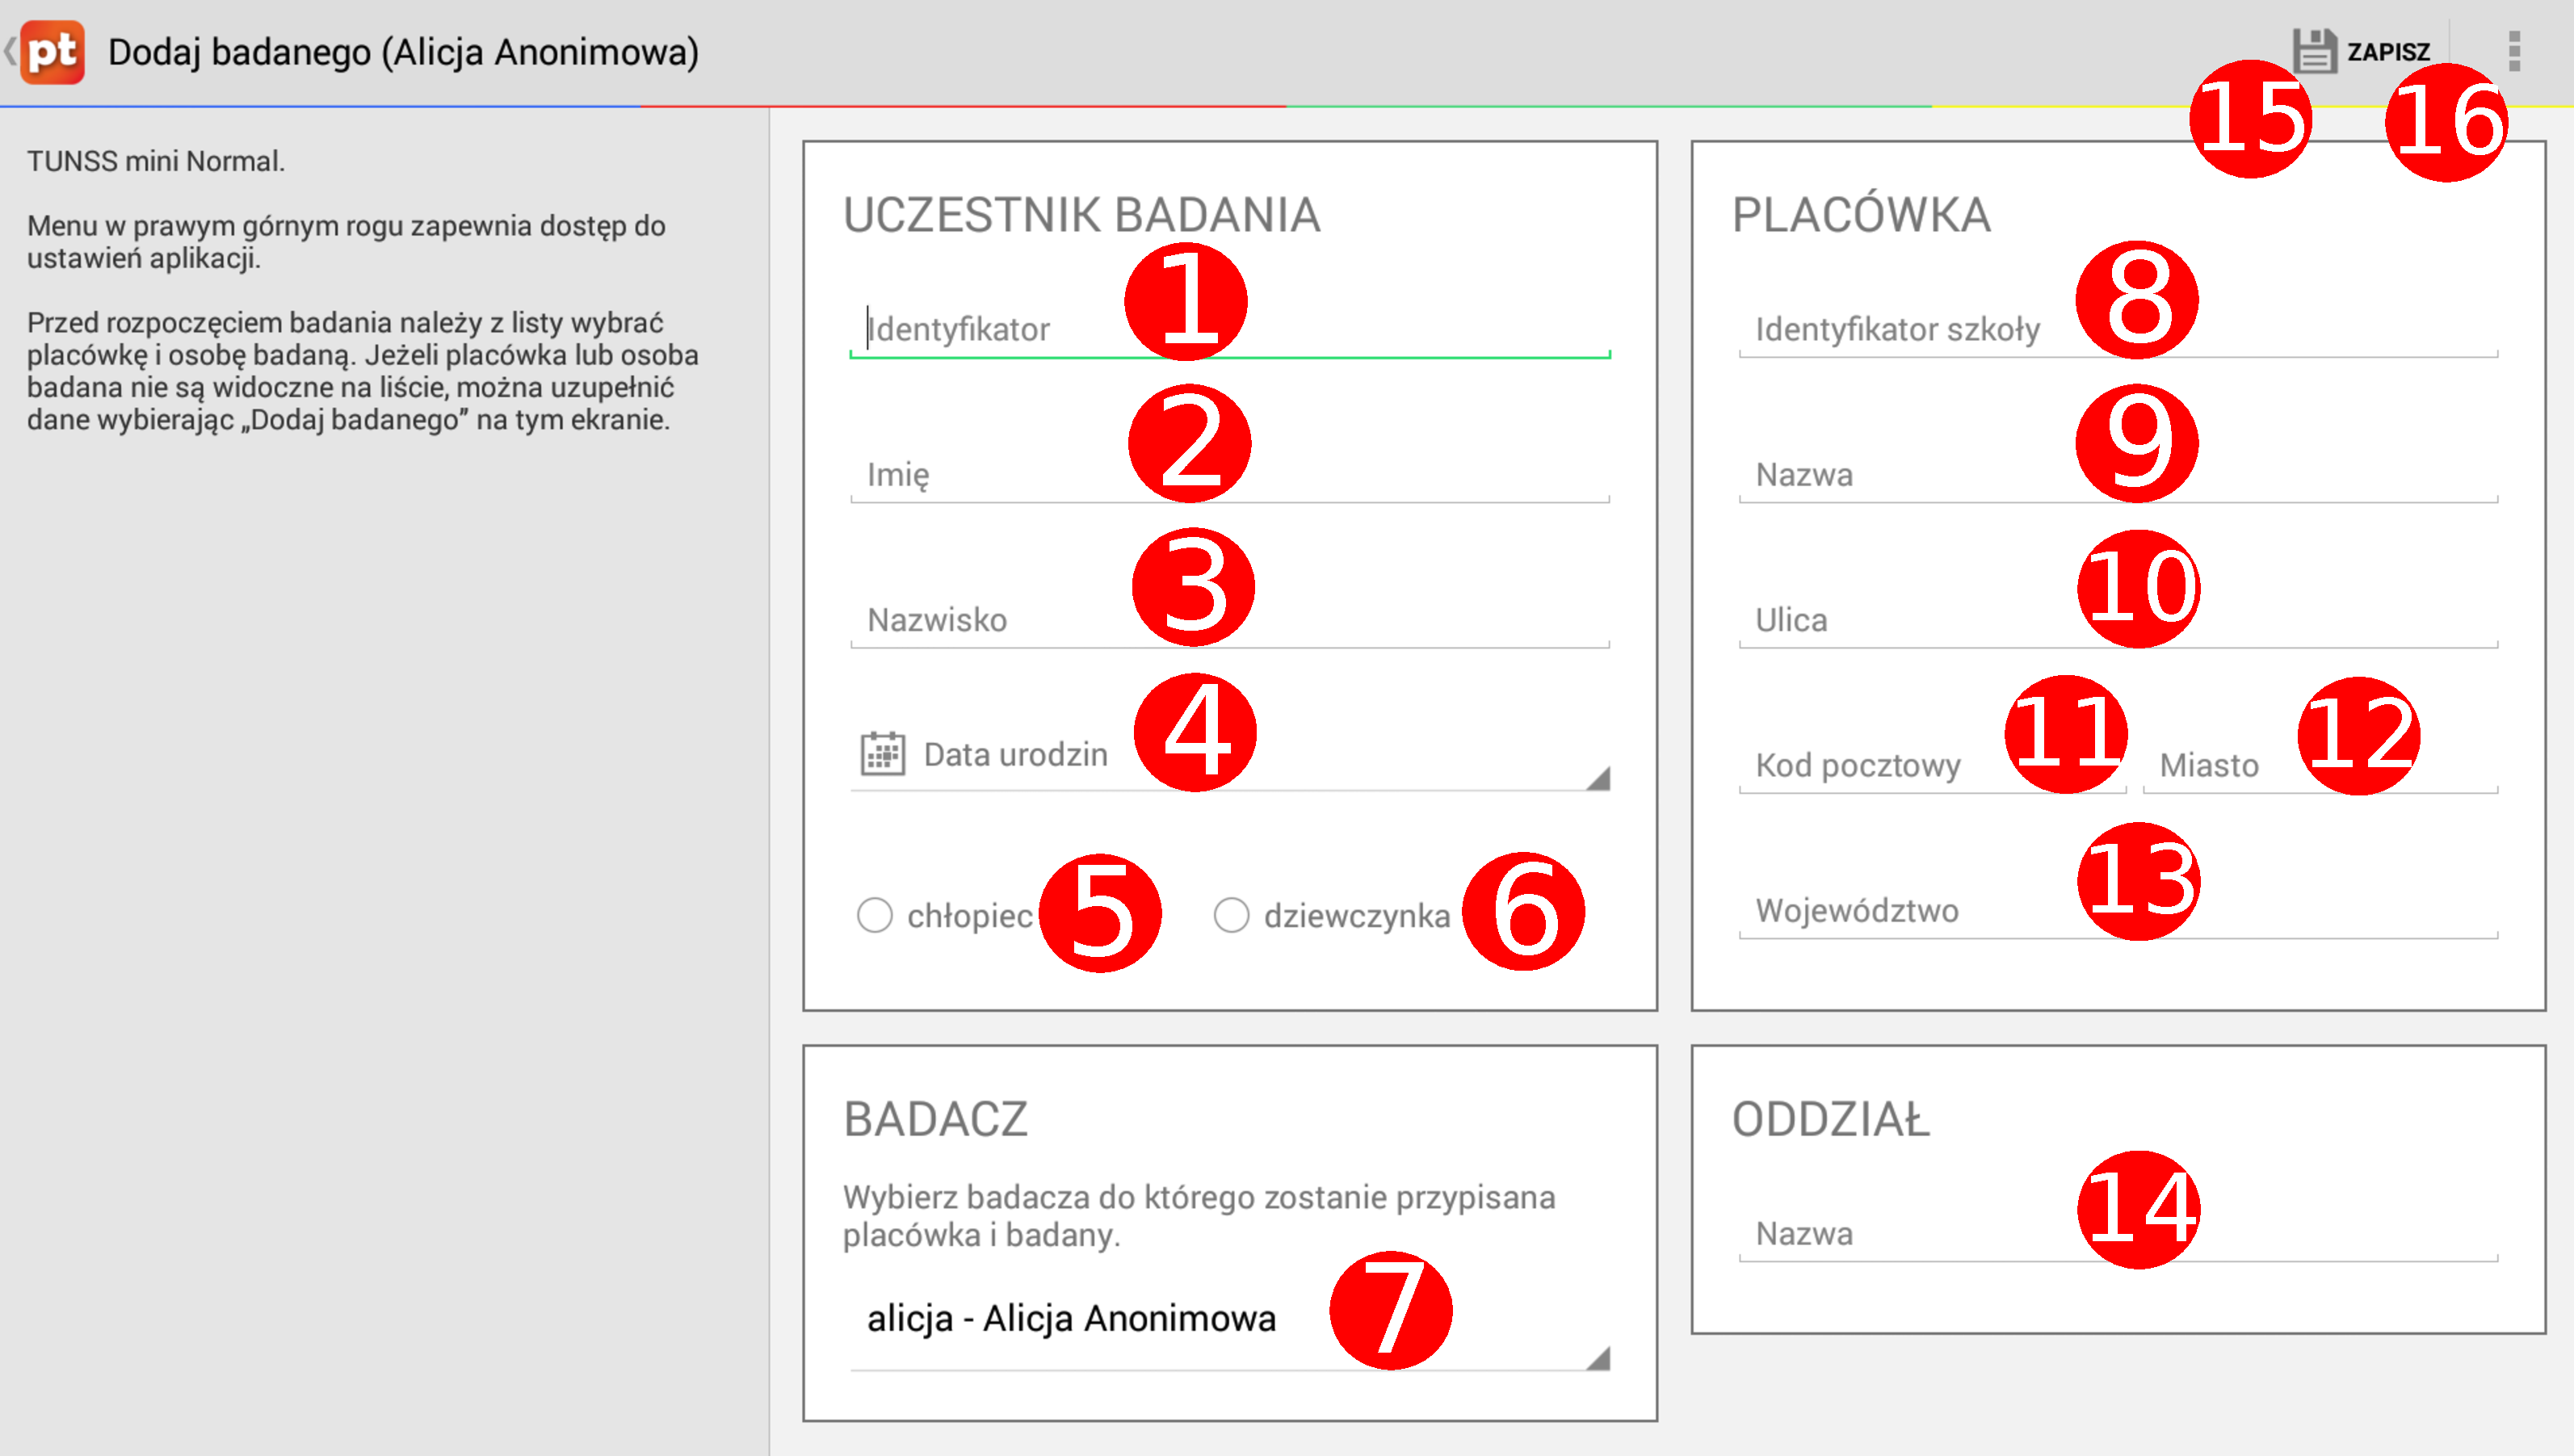
\includegraphics[width=0.96\textwidth]{activity_examinee_manager.pdf}
\caption{Ekran dodawania badanych}
\label{fig:examineemgr}
\end{figure}

Ekran dodawania badanych służy do wprowadzania danych nowych osób które mają zostać przebadane przy użyciu testu. Na tym ekranie znajdują się następujące pola (rysunek \ppref{fig:examineemgr}):

\begin{enumerate}
\item[(1)] Pole identyfikatora osoby badanej. Wartość tego pola powinna być unikatowa dla osoby badanej, odpowiednie jej ustawienie może też zostać wskazane przez operatora testu.
\item[(2)] Imię osoby badanej
\item[(3)] Nazwisko osoby badanej
\item[(4)] Data urodzin osoby badanej. Naciśnięcie pola powoduje pokazanie okna kalendarza za pomocą którego można wybrać dzień urodzin.
\item[(5)] Wybór płci osoby badanej - chłopiec
\item[(6)] Wybór płci osoby badanej - dziewczynka
\item[(7)] Wybór badacza, do którego zostanie przypisana badana osoba. To pole jest automatycznie ustawiane na aktualnie zalogowanego badacza, można jednak je zmienić by przypisać nowo dodawaną osobę do innego badacza.
\item[(8)] Identyfikator placówki osoby badanej. Wartość tego pola powinna być unikatowa dla danej szkoły, odpowiednie jej ustawienie może też zostać wskazane przez operatora testu.
\item[(9)] Nazwa placówki osoby badanej
\item[(10)] Adres placówki osoby badanej - ulica wraz z numerem
\item[(11)] Adres placówki osoby badanej - kod pocztowy
\item[(12)] Adres placówki osoby badanej - nazwa miasta
\item[(13)] Adres placówki osoby badanej - województwo
\item[(14)] Nazwa oddziału osoby badanej w placówce
\end{enumerate}

W przypadku gdy za pomocą tego okna dodano już wcześniej osobę z przypisaną placówką i/lub oddziałem, kafelki ``Placówka'' oraz ``Oddział'' zostają zastąpione listami wyboru, za pomocą których można od razu przypisać nową osobę do wcześniej zarejestrowanej jednostki. W celu przypisania nowej osoby do nowego oddziału lub placówki, należy wówczas w polu wyboru wskazać wartość ``Dodaj nowy''.

Oprócz pól, na ekranie znajdują się dwa przyciski: 

\begin{enumerate}
\item[(15)] Przycisk zapisu. Naciśnięcie go spowoduje sprawdzenie poprawności wprowadzonych danych, zapisanie danych osoby badanej oraz powrót do ekranu głównego.
\item[(16)] Przycisk menu. Menu tego ekranu zawiera jedną funkcję, ``Zgłoś błąd''. Naciśnięcie jej powoduje pokazanie okna zgłaszania błędów (rozdział \ppref{chap:bug_report}).
\end{enumerate}

Proszę zwrócić uwagę, że nie każdy rodzaj testu wymaga wypełnienia wszystkich pól. W przypadku braku wymaganych danych, aplikacja odmówi zapisania nowej osoby i wskaże które pola należy wypełnić.

\chapter{Ekran uruchamiania testu}
\label{chap:runtest}

\begin{figure}[b!]
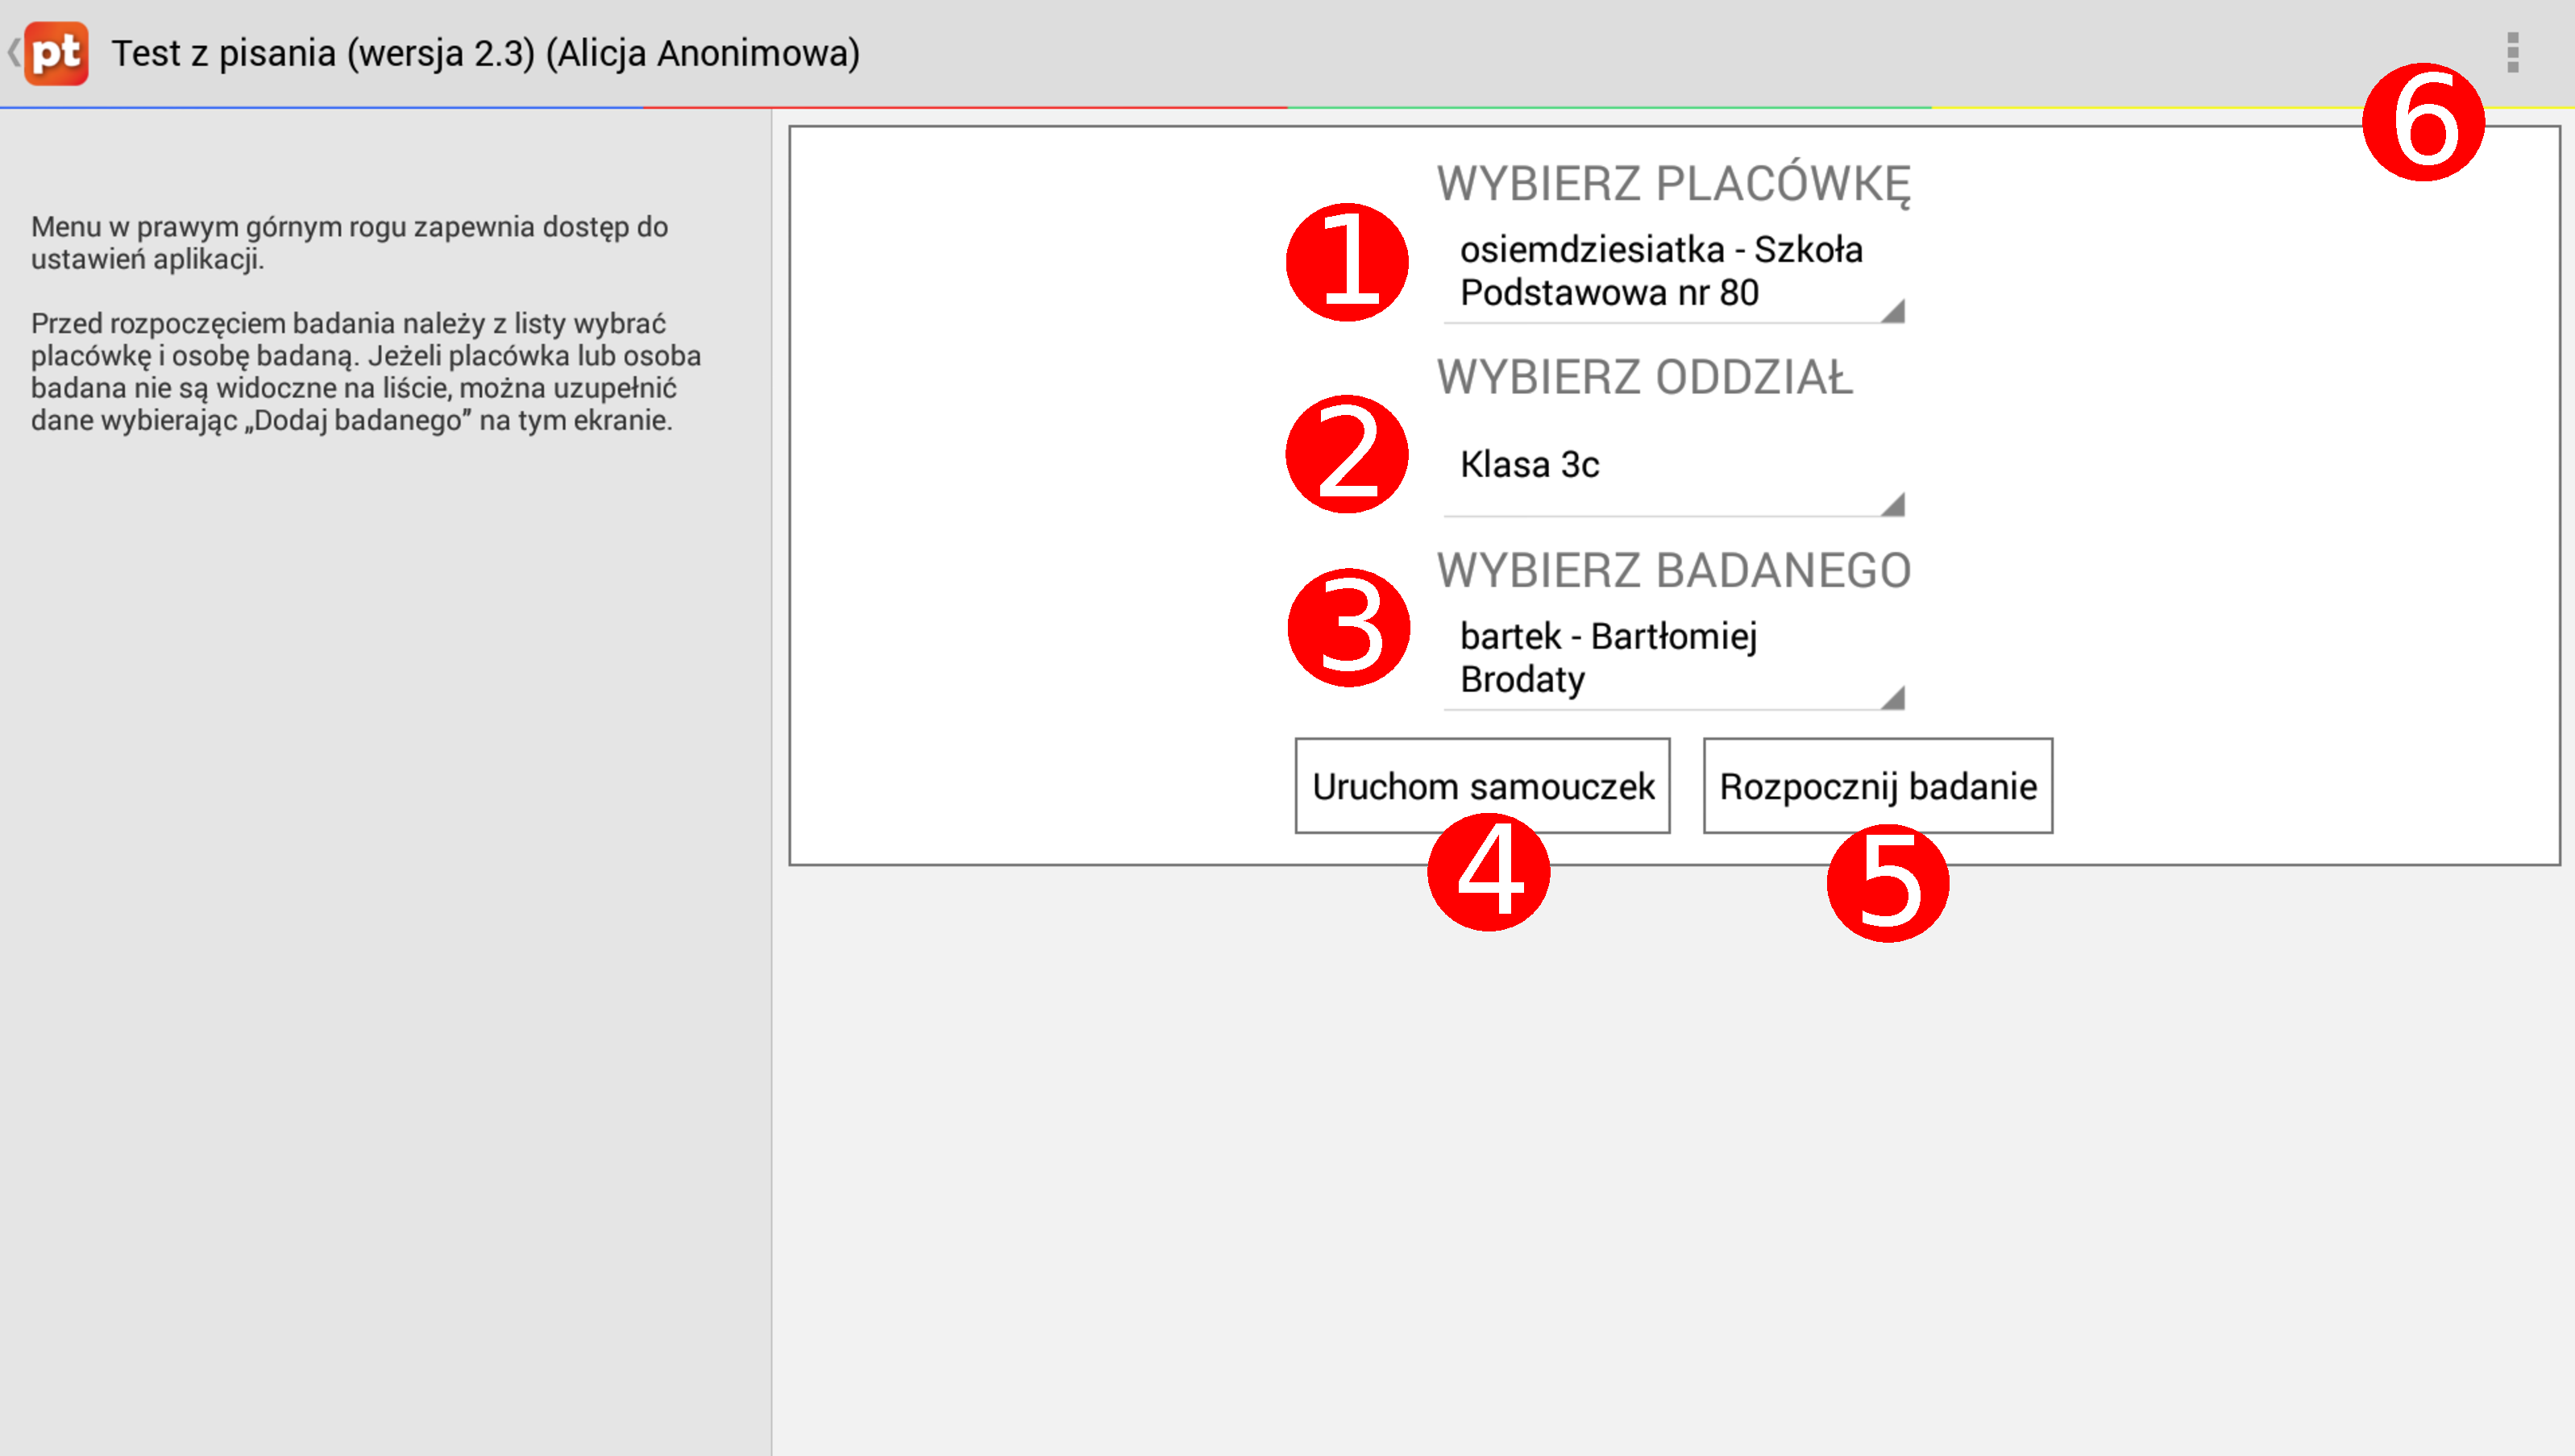
\includegraphics[width=0.96\textwidth]{activity_test_config.pdf}
\caption{Ekran uruchamiania testu}
\label{fig:runtest}
\end{figure}

Ekran uruchamiania testu służy do przygotowania badania. Na tym ekranie znajdują się następujące pola (rysunek \ppref{fig:runtest}):

\begin{enumerate}
\item[(1)] Wybór placówki - w tym polu należy wskazać placówkę do której przypisana jest osoba badana.
\item[(2)] Wybór oddziału - w tym polu należy wskazać oddział do którego przypisana jest osoba badana.
\item[(3)] Wybór osoby badanej - należy wskazać osobę, która będzie wykonywać test.
\end{enumerate}

Ekran posiada trzy przyciski:

\begin{enumerate}
\item[(4)] Przycisk uruchamiający samouczek - specjalny tryb testu przeznaczony do nauki obsługi testu przez osobę badaną. Więcej informacji o tym trybie znajduje się w rozdziale \pref{sec:test_pilotdemotutorial_tutorial}.
\item[(5)] Przycisk uruchamiający test - powoduje uruchomienie testu w trybie zwykłego badania.
\item[(6)] Przycisk menu. Menu tego ekranu zawiera jedną funkcję, ``Zgłoś błąd''. Naciśnięcie jej powoduje pokazanie okna zgłaszania błędów (rozdział \ppref{chap:bug_report}).
\end{enumerate}


\chapter{Ekran zadania}
\label{chap:test}

\begin{figure}[b!]
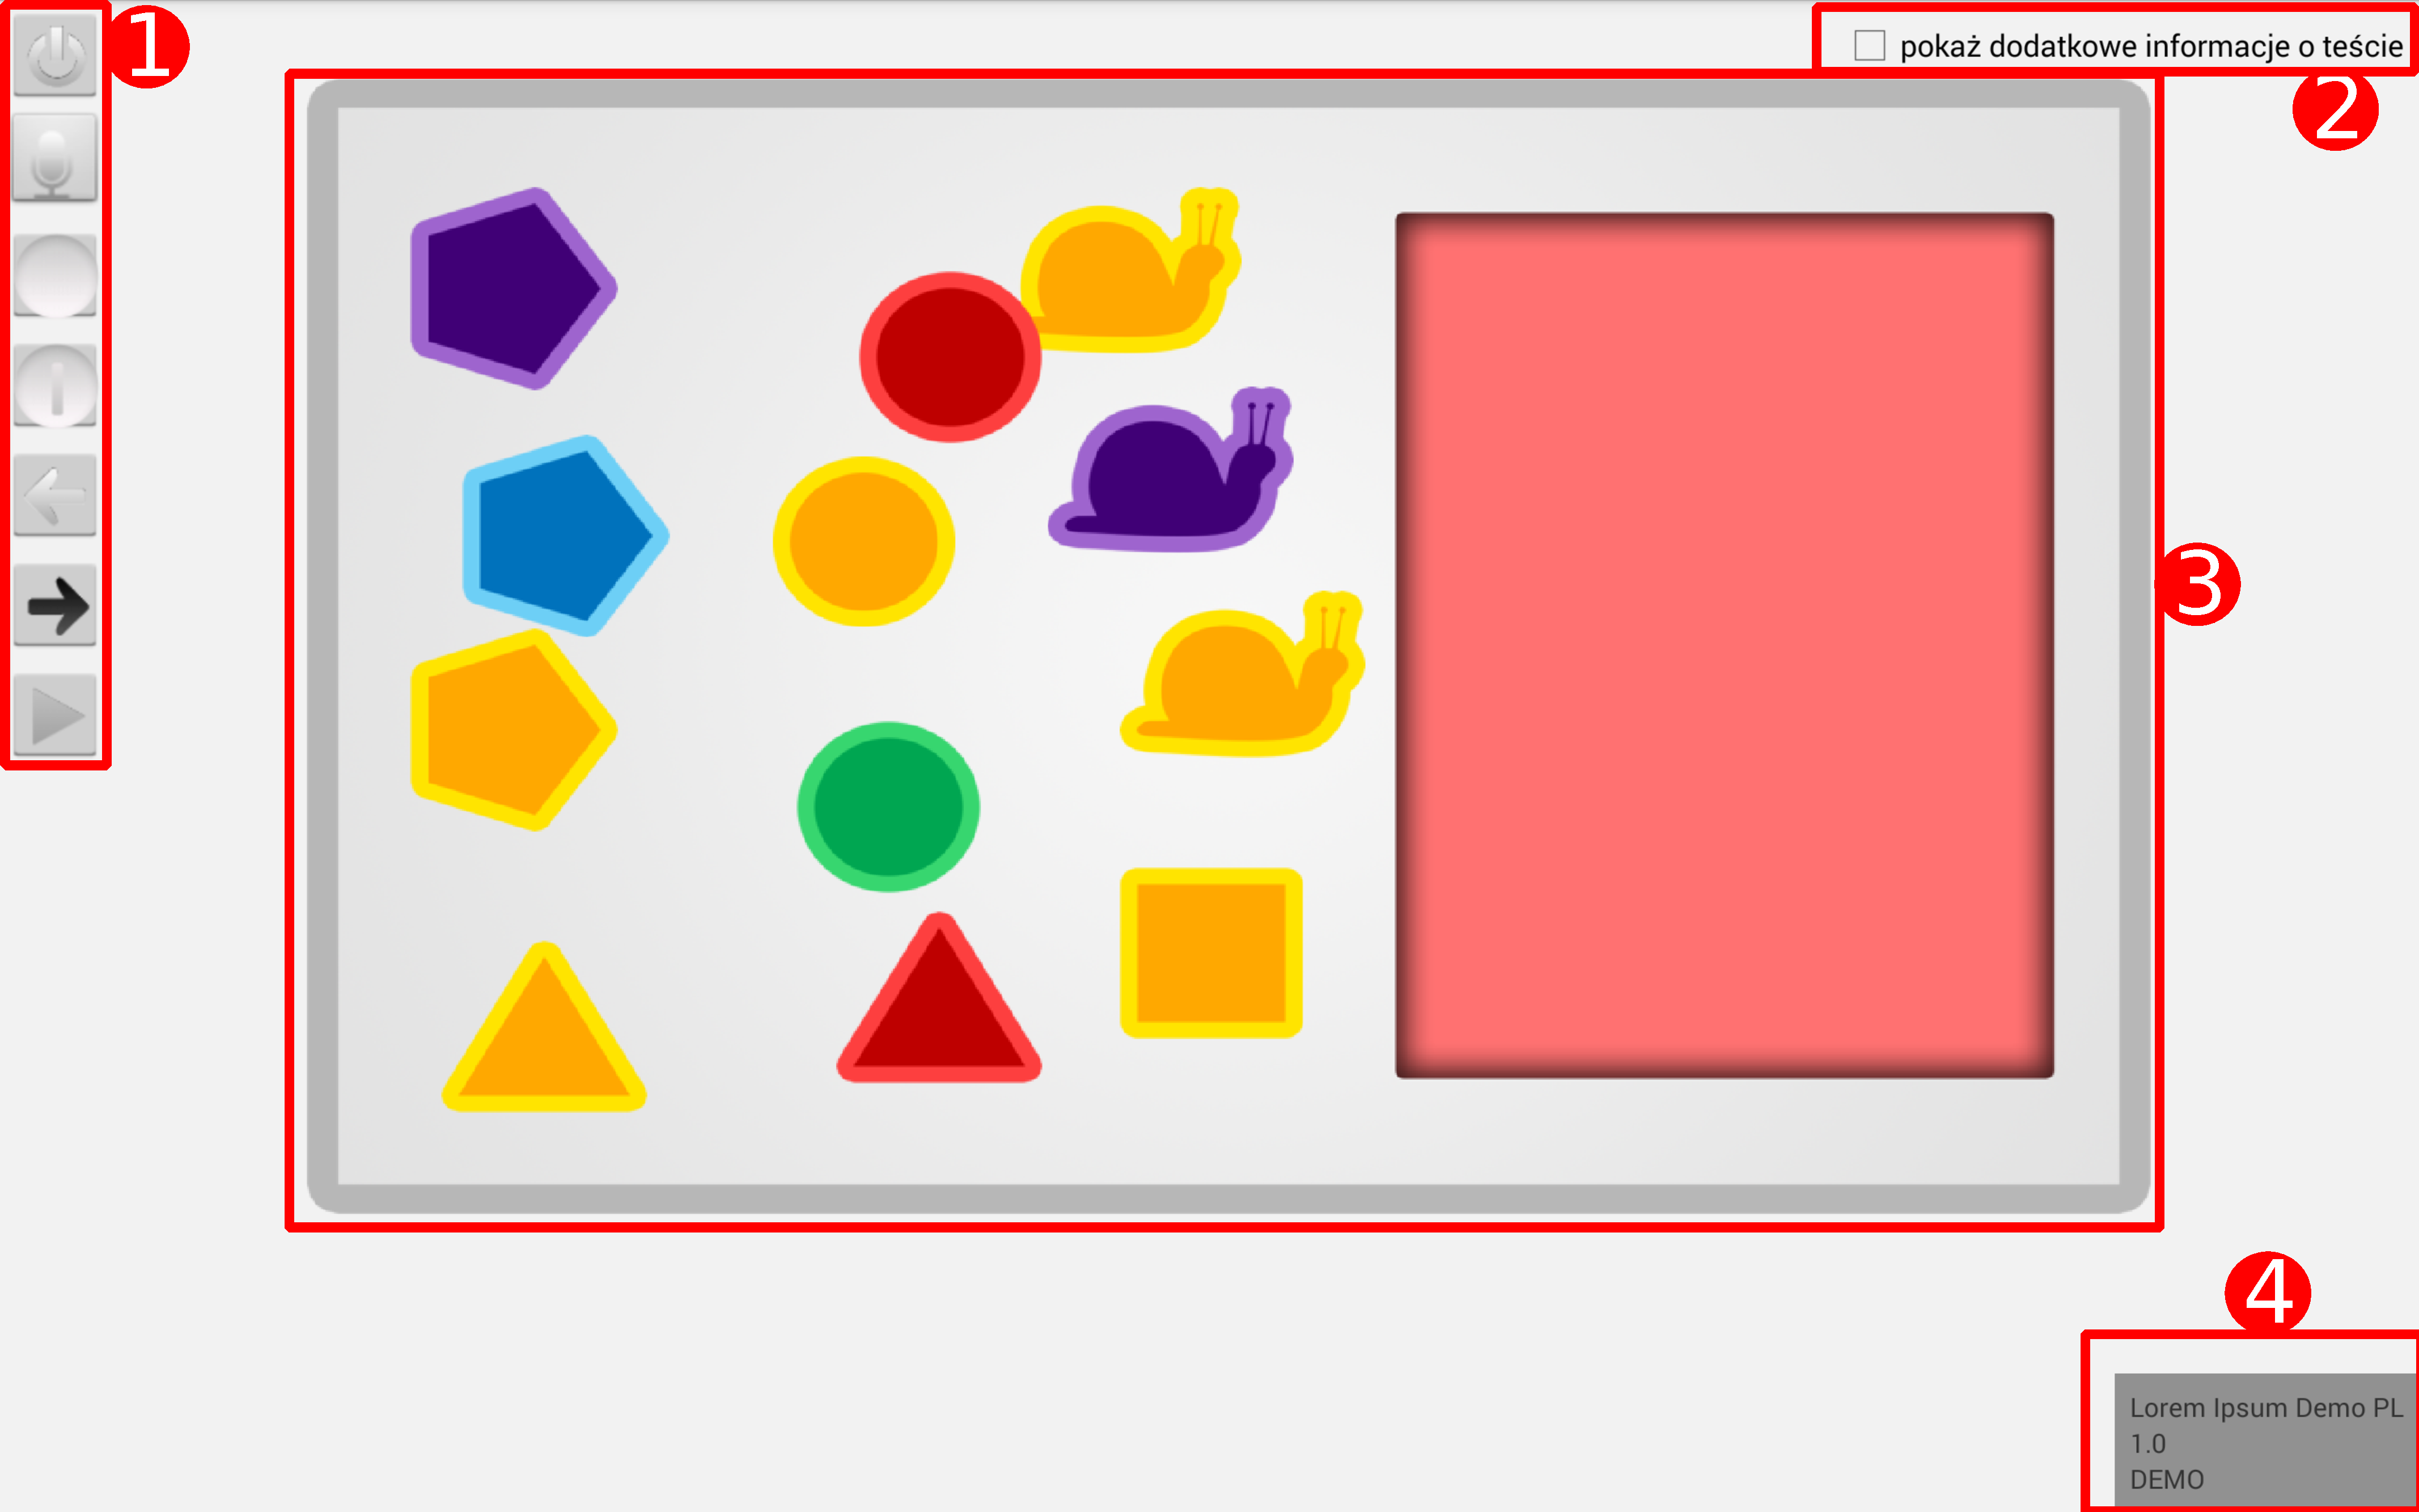
\includegraphics[width=0.96\textwidth]{test.pdf}
\caption{Ekran zadania}
\label{fig:test}
\end{figure}

Ekran zadania służy wyświetlaniu osobie badanej kolejnych zadań, oraz sterowania przez badacza przebiegiem testu. Składa się on z kilku części (rysunek \ppref{fig:test}):

\begin{enumerate}
\item[(1)] Przyciski sterujące przebiegiem testu
\item[(2)] Przycisk włączający wyświetlanie szczegółowych informacji o aktualnym zadaniu
\item[(3)] Plansza zadania, na której wyświetlana jest związana z nim zawartość. W przypadku niektórych zadań wyświetla ona obiekty reagujące na dotyk.
\item[(4)] Pole wyświetlające podstawowe informacje o aktualnie wykonywanym teście: jego nazwę, wersję oraz tryb pracy.
\end{enumerate}

Zawsze widoczne są jedynie elementy (1) i (3). Elementy (2) i (4) nie są widoczne podczas normalnych testów, a jedynie w specjalnych trybach pracy (patrz rozdział \ppref{sec:test_pilotdemotutorial}).

Podczas wyświetlania badania treść polecenia może być odtwarzania z głośnika urządzenia.


\section{Przyciski sterujące testem}
\label{sec:test_buttons}

Na pasku przycisków sterujących (rysunek \ppref{fig:test}, obszar 1) znajdują się różne przyciski sterujące aktualnym zadaniem oraz przebiegiem testu. Nie zawsze wszystkie przyciski są widoczne, zależy to od konfiguracji testu oraz aktualnie wyświetlanego zadania:

\newcommand{\buttonimage}[1]{
\includegraphics[scale=0.5]{#1}%	
}
\newcommand{\button}[2]{
\buttonimage{#1} & \parbox[b][2em][c]{0.8\textwidth}{#2} \\%
}
\newcommand{\buttons}[2]{
#1 & \parbox[b][2em][c]{0.8\textwidth}{#2} \\%
}

\noindent
\begin{tabularx}{\textwidth}{rl}
\button{button_quit.png}{Wyjście z badania. Powoduje wyświetlenie prośby o potwierdzenie a następnie okna umożliwiającego dodanie notatki (rozdział \ppref{sec:test_note})}
\button{button_previous.png}{Przejście do poprzedniego zadania}
\button{button_next.png}{Przejście do kolejnego zadania}
\button{button_command.png}{Ponowne odtworzenie treści polecenia}
\button{button_step.png}{Przejście do kolejnego etapu zadania}
\button{button_microphone.png}{Włączenie/wyłączenie nagrywania dźwięku}
\button{button_camera.png}{Wykonanie zdjęcia przy pomocy aparatu fotograficznego w urządzeniu}
\button{button_manual_mark.png}{Zastąpienie automatycznej oceny oceną wystawioną przez badacza}
\buttons{\buttonimage{button_mark_zero.png}\buttonimage{button_mark_one.png}\buttonimage{button_mark_two.png}\buttonimage{button_mark_many.png}}{Wystawienie oceny, odpowiednio 0 (zero), 1 (jeden), 2 (dwa) lub więcej punktów}
\button{button_reload.png}{Ponowne uruchomienie zadania}
\end{tabularx}

Użycie niektórych przycisków wymaga długiego przytrzymania. Ma to na celu ograniczenie możliwości przypadkowego aktywowania przycisków przez osobę badaną.


\section{Notatka do badania}
\label{sec:test_note}

\begin{wrapfigure}{r}{0.5\textwidth}
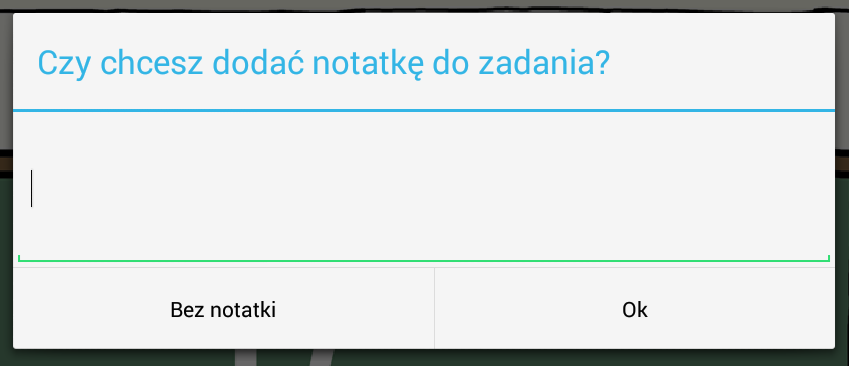
\includegraphics[width=0.48\textwidth]{test-note.png}
\caption{Okno notatki do badania}
\vspace{-10pt}
\label{fig:test_note}
\end{wrapfigure}


Przy opuszczaniu testu, użytkownik zostaje zapytany o potwierdzenie zamiaru opuszczenia testu. Ma to na celu uniknięcie niecelowego zakończenia badania. Gdy użytkownik potwierdzi zamiar, wyświetlone zostanie okno notatki (rysunek \ppref{fig:test_note}). W tym miejscu badacz może wprowadzić dodatkowe informacje związane z przeprowadzanym badaniem. Wybranie przycisku ``Ok'' spowoduje zapisanie wprowadzonej notatki wraz z wynikami badania, a ``Bez notatki'' - porzucenie ich.


\section{Tryb pilotażowy, demonstracyjny i samouczek}
\label{sec:test_pilotdemotutorial}

Oprócz normalnego trybu pracy, uruchamianego za pomocą przycisku ``Rozpocznij badanie'' (rysunek \ppref{fig:runtest}, przycisk 5), możliwe jest uruchomienie testu w kilku innych trybach. Charakteryzują się one różnicami w zakresie kolejności wyświetlania zadań oraz ilości informacji prezentowanych na ekranie.

\subsection{Tryb demonstracyjny}
\label{sec:test_pilotdemotutorial_demo}

Celem trybu demonstracyjnego jest zapoznanie osób niezaznajomionych z aplikacją lub konkretnym bankiem zadań z ich możliwościami i zawartością. Nie służy on do przeprowadzania właściwych badań. Zadania wyświetlane są w uprzednio zdefiniowanej kolejności, a ich wyniki nie są nigdzie gromadzone.

W aplikacji istnieją dwa rodzaje paczek zadań demonstracyjnych - wbudowane w aplikację i dostarczane wraz z bankami zadań. Te pierwsze, są zawsze dostępne i prezentują możliwości aplikacji (istnieją dwie wersje językowe: polska i angielska). Te drugie dostarczane są przez autorów lub dystrybutorów poszczególnych banków zadań i pojawiają się w aplikacji w wyniku instalacji banku zadań przez jednego z badaczy posiadających konto na tym urządzeniu.

Uruchomienie trybu demo możliwe jest na dwa sposoby:
\begin{enumerate}
\item[1] Poprzez wybranie przycisku ``Demo'' na ekranie logowania (rysunek \ppref{fig:login}, przycisk 3). Po naciśnięciu przycisku, pojawia się lista wszystkich obecnych w urządzeniu paczek demo (rysunek \ppref{fig:login_demo_list}). Wybranie jednej z pozycji na liście powoduje uruchomienie danego testu w trybie demonstracyjnym.
\item[2] Poprzez wybranie przycisku ``Wersja demonstracyjna'' na ekranie głównym (rysunek \ppref{fig:main}, przycisk 4). W tym wypadku uruchomiony zostaje tryb demonstracyjny dla aktualnie uruchomionego przez badacza banku zadań. W przypadku gdy bank zadań nie dostarcza paczki zadań demonstracyjnych, przycisk jest wyszarzony.
\end{enumerate}

Niezależnie od sposobu uruchomienia, na ekranie pojawia się zwykły ekran zadania (rysunek \ppref{fig:test}). W trybie demonstracyjnym widoczne są wszystkie elementy - w tym przycisk włączający widok szczegółowych informacji oraz pole z nazwą uruchomionego testu.

Po opuszczeniu ekranu zadania, następuje automatyczne przejście do ekranu raportu demonstracyjnego. W związku z tym że wyniki w trybie demo nie są zbierane, wyświetlany raport opiera się zasadniczo na danych losowych lub sztucznie dobranych. Szerszy opis raportu w trybie demo znajduje się w rozdziale \pref{sec:report_demo}.


\subsection{Tryb samouczka}
\label{sec:test_pilotdemotutorial_tutorial}

Tryb samouczka przeznaczony jest do zapoznawania z aplikacja i testem osób badanych, które wcześniej w nim nie uczestniczyły. Celem jest nauczenie obsługi typowych dla danego banku zadań elementów, tak by zredukować wpływ nieznajomości obsługi testu na wyniki badań. Samouczek, podobnie jak demo, nie służy do przeprowadzania właściwych badań. Zadania wyświetlane są w uprzednio zdefiniowanej kolejności, a ich wyniki nie są nigdzie gromadzone.

Tryb samouczka jest ściśle związany z bankiem zadań. Uruchamiany jest poprzez przycisk ``Uruchom samouczek'' na ekranie uruchamiania testu (rysunek \ppref{fig:runtest}, przycisk 4).

Po naciśnięciu przycisku, na ekranie pojawia się zwykły ekran zadania (rysunek \ppref{fig:test}). W trybie samouczka widoczne jest pole z nazwą uruchomionego testu, może być również widoczny przycisk włączający widok szczegółowych informacji.

Po dojściu do ostatniego zadania w trybie samouczka, następuje automatyczne przejście do właściwego badania. Od tego momentu działają wszystkie reguły dla zwykłego badania.

\subsection{Tryb pilotażowy}
\label{sec:test_pilotdemotutorial_pilot}

Tryb pilotażu jest trybem szczególnym - nie posiada on żadnej odpowiadającej sobie opcji w interfejsie aplikacji. Jest on definiowany wewnątrz banku zadań i nie może zostać wyłączony przez użytkownika. Tryb ten ma na celu ułatwienie przeprowadzania pilotażowym etapów badań z użyciem nowych banków zadań.

Użycie trybu pilotażu jest możliwe wyłącznie w specjalnie zdefiniowanych \emph{pilotażowych} wersjach banków zadań. Instalacja takiego banku przebiega w zwykły sposób, a odróżnienie od standardowego banku widoczne jest na ekranie wyboru banku zadań (rysunek \ppref{fig:suiteselect}) - wersje pilotażowe mają automatycznie dodany przypis ``pilotażowy bank zadań''.

W celu aktywacji pilotażowego banku zadań, należy wybrać go z listy zainstalowanych banków zadań. W trybie pilotażowym uruchomienie testu następuje w zwykły sposób - poprzez wybranie przycisku ``Rozpocznij badanie'' na ekranie uruchamiania testu (rysunek \ppref{fig:runtest}, przycisk 5).

W trybie pilotażowym na ekranie zadania (rysunek \ppref{fig:test}) widoczne jest pole z nazwą uruchomionego testu, zależnie od decyzji operatora banku zadań widoczny być może też przycisk włączający widok szczegółowych informacji.

Zasadniczo badanie w trybie pilotażowym przeprowadzane jest w zwykły sposób. Główną różnicą, oprócz rozszerzonego zestawu elementów na ekranie, jest działanie funkcji rejestracji dźwięku - podczas gdy w zwykłym badaniu nagrywanie dźwięku w niektórych zadaniach można aktywować poprzez użycie przycisku mikrofonu, w trybie pilotażu nagrywanie jest uruchamianie automatyczne, wraz z wyświetleniem zadania które je umożliwia.


\chapter{Ekran raportu}
\label{chap:report}

\begin{figure}[b!]
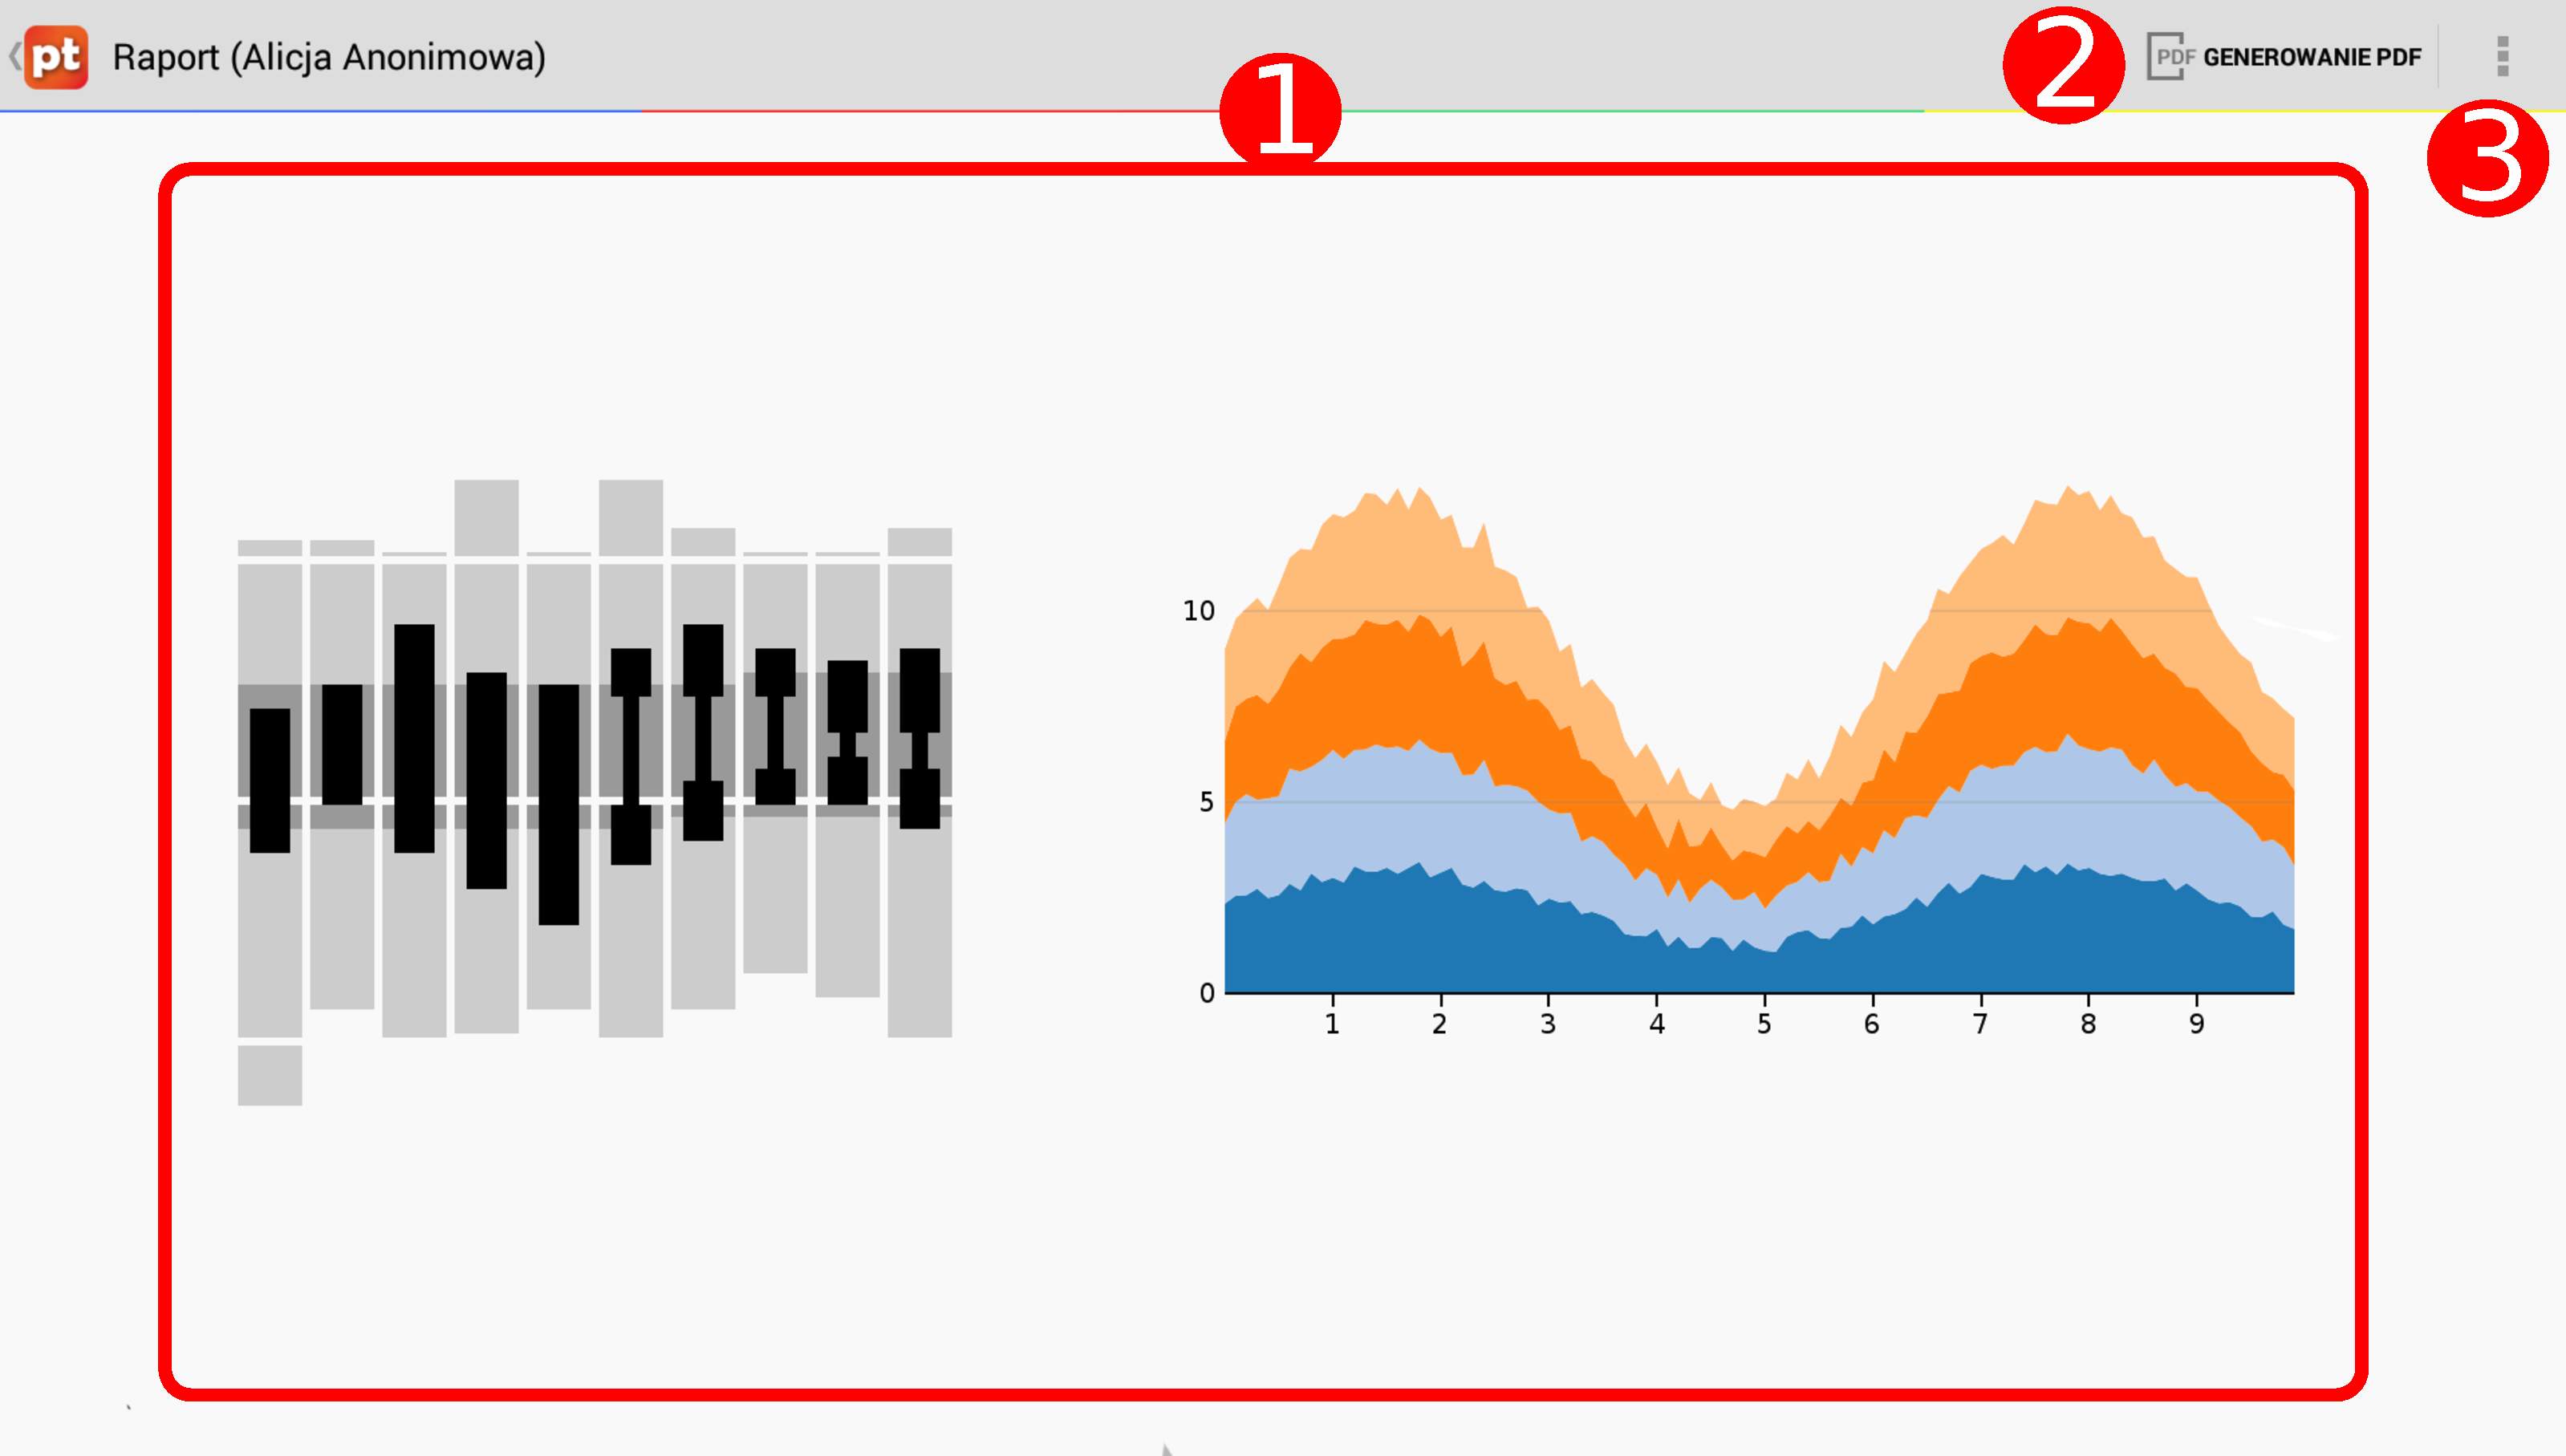
\includegraphics[width=0.96\textwidth]{report.pdf}
\caption{Ekran raportu}
\label{fig:report}
\end{figure}

Ekran raportu służy prezentacji rezultatów zgromadzonych badań. Jest on podzielony na kilka cześci (rysunek \ppref{fig:report}):

\begin{enumerate}
\item[(1)] Przestrzeń raportu - miejsce w którym prezentowana jest treść raportu. Może zawierać elementy interaktywne oraz korzystać z danych referencyjnych przygotowanych przez autorów banku zadań.
\item[(2)] Przycisk generowania plików PDF. Po jego naciśnięciu otwiera się menu z kilkoma opcjami (patrz rozdział \ppref{sec:report_pdf})
\item[(3)] Przycisk menu. Menu tego ekranu zawiera jedną funkcję, ``Zgłoś błąd''. Naciśnięcie jej powoduje pokazanie okna zgłaszania błędów (rozdział \ppref{chap:bug_report}).
\end{enumerate}


\section{Generowanie plików PDF}
\label{sec:report_pdf}

\begin{wrapfigure}{l}{0.5\textwidth}
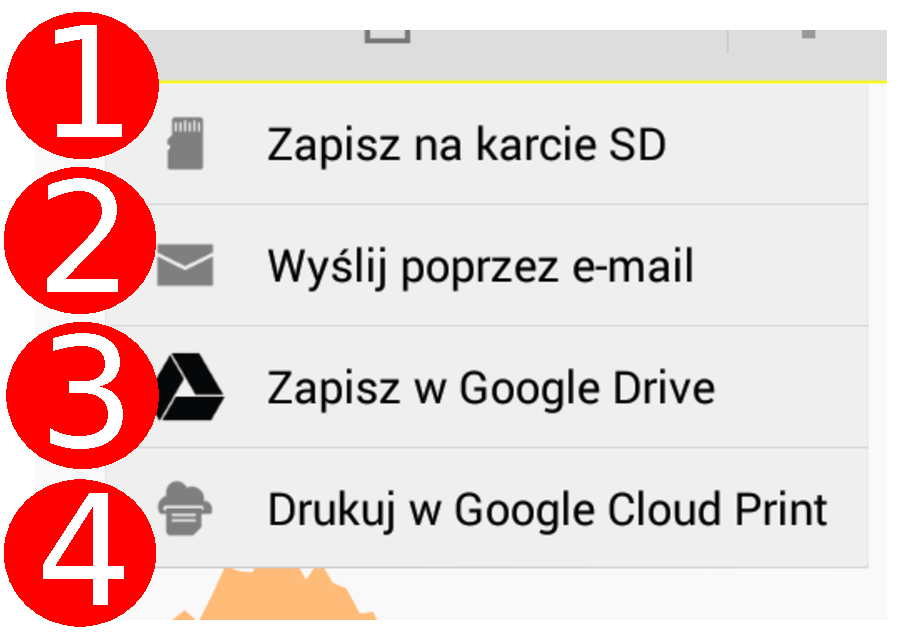
\includegraphics[width=0.48\textwidth]{report_pdfmenu.pdf}
\caption{Menu ``Generowanie PDF''}
\label{fig:report_pdfmenu}
\end{wrapfigure}

Funkcję generowania plików PDF aktywuje się poprzez przycisk ``Generowanie PDF'' na ekranie raportu (rysunek \ppref{fig:report}, przycisk 2). Po jego naciśnięciu, na ekranie pojawi się okno ze szczegółowymi możliwościami (rysunek \ppref{fig:report_pdfmenu}):

Przycisk zapisu raportu na kartę SD (1) powoduje wygenerowanie pliku PDF, a następnie zapisanie go na karcie SD urządzenia. Po naciśnięciu przycisku przez chwilę widoczny jest komunikat o generowaniu, a następnie wyświetlana jest nazwa pliku w którym zapisano raport.

Przycisk wysyłania raportu poprzez e-mail (2) daje możliwość wysłania raportu w postaci pliku PDF poprzez pocztę elektroniczną. Po naciśnięciu przycisku przez chwilę widoczny jest komunikat o generowaniu, a następnie utworzenie wiadomości w wybranym kliencie e-mail wraz z raportem w formacie PDF jako załącznikiem.

Przycisk zapisywania raportu w usłudze Google Drive (\emph{Dysk Google}) (3) daje możliwość zapisu raportu bezpośrednio na konto użytkownika tej usługi. Po naciśnięciu przycisku przez chwilę widoczny jest komunikat o generowaniu, a następnie następuje połączenie z usługą Google Drive i zapis pliku we wskazanym miejscu.

Przycisk drukowania raportu przy użyciu usługi Google Cloud Print (4) daje możliwość natychmiastowego druku raportu na drukarce podłączonej do tej usługi. Po naciśnięciu przycisku przez chwilę widoczny jest komunikat o generowaniu, a następnie następuje połączenie z usługą Google Cloud Print i wydruk raportu na wskazanej drukarce.

W związku z tym że raport może zawierać elementy interaktywne, wygenerowany plik PDF może różnić się od raportu widocznego na ekranie.


\section{Raport demonstracyjny}
\label{sec:report_demo}

Raport demonstracyjny jest uruchamiany automatycznie po opuszczeniu ekranu zadań w trybie demo (rozdział \ppref{sec:test_pilotdemotutorial_demo}). Różni się on od zwykłego raportu brakiem danych związanych z badaniami. W związku z tym prezentuje on zawsze dane  niezależne od testów wykonanych przy użyciu urządzenia. Mogą być one losowe, bądź celowo dobrane przez autora tak, by ukazać różne aspekty działania danego raportu.

W pozostałych aspektach, działa i wygląda on identycznie do zwykłego raportu - elementy interaktywne zachowują się w identyczny sposób, jest również możliwe wygenerowanie z niego pliku PDF.


\chapter{Ekran zgłaszania błędów}
\label{chap:bug_report}

Ekran zgłaszania błędów służy do wysyłania zgłoszeń dotyczących nieprawidłowości w pracy aplikacji bądź napotkanych problemów z jej obsługą. Wywołać można go z każdego ekranu, za wyjątkiem ekranu zadania. Na większości ekranów uruchamia się go z menu aktywowanego przyciskiem w prawym górnym rogu ekranu (np. rysunek \ppref{fig:suiteselect}, przycisk 2 lub \ppref{fig:main} przycisk 5). Na ekranie głównym uruchamia się go przyciskiem ``Zgłoś błąd'' w prawym dolnym rogu ekranu (rysunek \ppref{fig:login}, przycisk 6).

\begin{wrapfigure}{r}{0.5\textwidth}
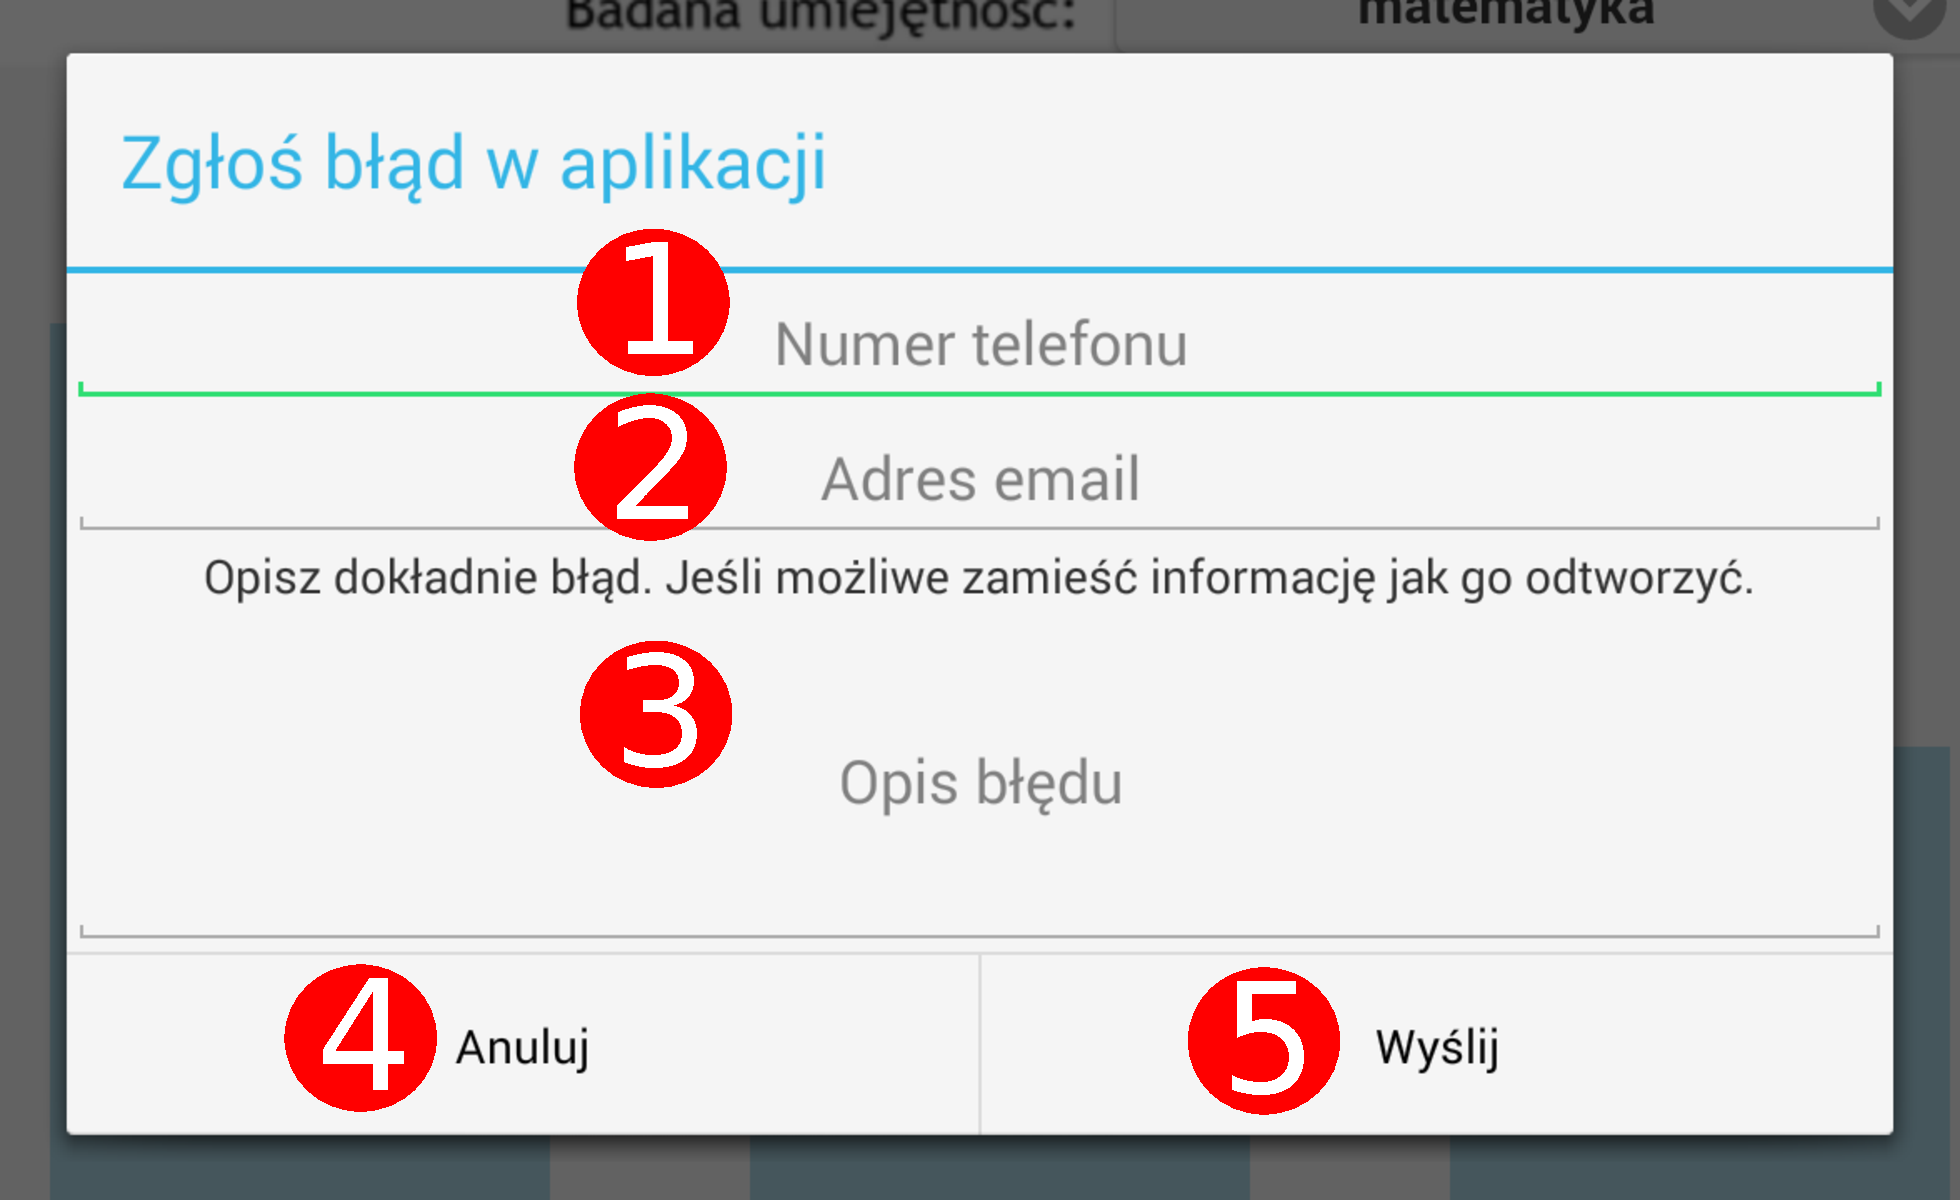
\includegraphics[width=0.48\textwidth]{window_report_bug.pdf}
\caption{Okno zgłaszania błędów}
\label{fig:bug_report}
\end{wrapfigure}

W celu zgłoszenia informacji o błędzie, należy wypełnić pola w sposób następujący (rysunek \ppref{fig:bug_report}):

(1) Numer telefonu osoby zgłaszającej błąd. Zostanie on użyty w celu nawiązania kontaktu dla ustalenia szczegółów pojawiającego się błędu.

(2) Adres e-mail osoby zgłaszającej błąd. Zostanie on użyty w celu nawiązania kontaktu dla ustalenia szczegółów pojawiającego się błędu.

(3) Opis błędu. Powinien być to krótki i przejrzysty opis zgłaszanej nieprawidłowości w działaniu aplikacji. Jeżeli błąd jest łatwo powtarzalny, opis powinien zawierać kolejne kroki w aplikacji prowadzące do jego wystąpienia.

(4) Przycisk wyjścia. Użycie go spowoduje że raport nie zostanie wysłany.

(5) Przycisk wysłania raportu. Po jego użyciu wyświetlony zostanie komunikat o przyjęciu zgłoszenia i informacje kontaktowe z obsługą techniczną. Użytkownik może ich użyć w celu kontaktu z obsługą techniczną, o ile ta nie skontaktuje się w nim w ciągu oznaczonego czasu.

\listoffigures

\end{document}